% Chapter 5

\begin{savequote}[45mm]
There are no significant technical limitations
to column temperature programming in the
order of a few hundred degrees per minute and
equally rapid cool-down rates.
\qauthor{Wolfgang Bertsch, pessimist, 1997}
\end{savequote}

\chapter{Instrumentation: Fast temperature programmed gas chromatography} % Main chapter title

\label{Chapter5} % For referencing this chapter elsewhere, use \ref{Chapter5}


This thesis discusses the development of a comprehensively coupled
(supercritical fluid × gas) chromatograph and its application to the analysis of
biodiesel. The discussion on the experimental work divides naturally into two
parts: the previous chapter discusses the supercritical fluid chromatography
(SFC) and this chapter discusses the gas chromatography (GC).


\section{Speed of analysis}

In principle, comprehensively coupled chromatography (as discussed in Section
\ref{sec:SFCxGC}) can be performed by manually or mechanically collecting
equal-sized fractions from a \textsuperscript{1}D chromatograph, and then
injecting a portion of each fraction into a different (\textsuperscript{2}D)
chromatograph. This will meet all the criteria for comprehensively coupled
chromatography.In practice, such an approach would be slow, labour-intensive,
expensive, and error-prone.

But reliable devices were invented that can repeatedly collect and re-inject
fractions of eluate \textit{while the \textsuperscript{1}D chromatograph is
still running}. These devices became known as \textit{modulators} and made
comprehensively coupled chromatography practical. Today GC×GC is an established
technique: the annual GC×GC Symposium is in its 15th year, and major reviews are
published regularly \autocite{Seeley2013,Prebihalo2018}.

In GC×GC the entire 2D chromatogram is finished within the duration of the
\textsuperscript{1}D run. This is made possible by using short, narrow-bore
columns with thin-film stationary phases in the \textsuperscript{2}D separation,
which allows \textit{fast chromatography}.

In LC×GC and SFC×GC with packed \textsuperscript{1}D columns using stopped-flow
modulation (as described in Section \ref{sec:stopflow}) the total run time can
be longer, but not indefinitely longer. Firstly, diffusion is not zero in dense
mobile phases so the stopped-flow time should be minimized to prevent
unnecessary peak broadening. Secondly, total run times must be practical: while
it's not inconceivable to have experiments that run for days, developing complex
instrumentation can reliably run for such long periods becomes expensive.

The time it takes for a stopped-flow SFC×GC run can be calculated from

\[t_{T} = t_{SFC} + \frac{t_{SFC}}{t_{m}} \times t_{GC}\]

where \(t_T\) is the total time, \(t_{SFC}\) is the time the unmodulated SFC run
would take, \(t_m\) is the modulation period, and \(t_{GC}\) is the time for
each GC run.

Examining the expression shows that we can decrease \(t_T\) by increasing
\(t_m\), but there is limit to this: if the modulation time becomes to long, the
separation obtained in the \textsuperscript{1}D separation might be lost, which
would mean it could no longer be considered comprehensively coupled
chromatography.

So the only way to decrease the total run times is to reduce \(t_{GC}\), the GC
run time.

For example, if a typical SFC run takes 20 minutes, and fractions are collected
for every 5 seconds of SFC run, it means there will be 20*60/5 = 240 fractions
collected. Each of these fractions must be injected into a GC chromatograph. If
each GC run took 1 minute, the SFC×GC run would last 240 minutes = 4 hours. Run
times this long is not unheard of in analytical chromatography, but it becomes
impractical.

This discussion should make it clear that for successful SFC×GC the GC
must be \textit{fast}.

\section{Fast gas chromatography theory}

The theory of fast gas chromatography has been well developed\todo{autocite
Blumberg1997-Blumberg1999}, and every chromatographer who has looked into faster
chromatography has met the chromatographer's trilemma (See Figure
\ref{fig:trilemma}): Any chromatographic method that involves trade-offs between
speed, resolution, and capacity can maximize only one at a time\footnote{This
trilemma applies only to capillary chromatography. When using packed columns the capacity
can be readily increased by using a column with a larger diameter and a larger
amount of packing.}. The fastest chromatogram will have low capacity and low
resolution, the highest resolution chromatogram will be slow and with low
capacity, and the chromatogram of a sample with a high concentration of analyte
will be slow and have low resolution \autocite{Klee2002}.

\begin{figure}
\centering
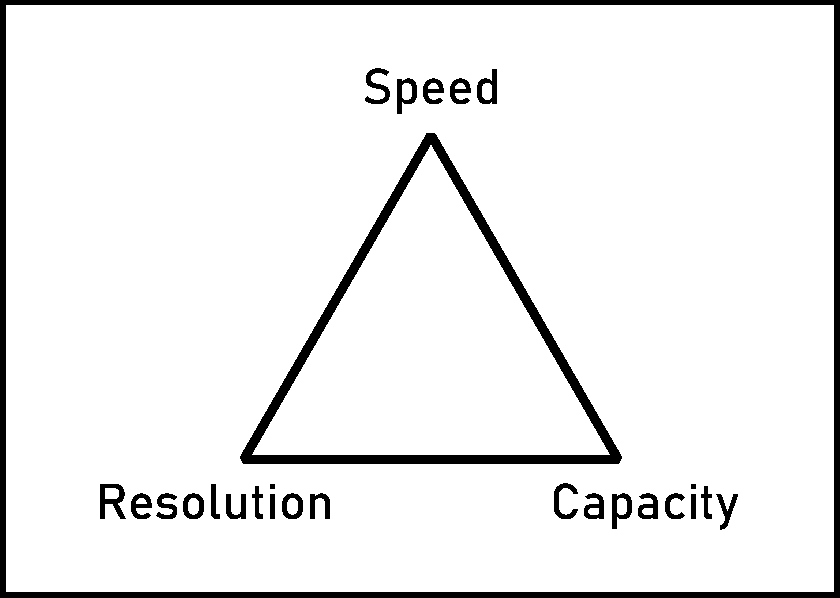
\includegraphics[width=0.75\textwidth]{Figures/Triangle.pdf}
\decoRule
\caption[Schematic diagram of a the chromatograher's trilemma.]{The chromatographer's trilemma.}
\label{fig:trilemma}
\end{figure}

We avoided the trilemma by not bothering with optimizing column capacity. Sample
capacity in capillary GC is a function of film thickness and column diameter. We
decided to use the workhorse of GC, the \SI{0.25}{\milli\metre} internal
diameter column with a \SI{0.25}{\micro\metre} film thickness. The stationary
phase was a proprietary cross-linked polysiloxane polymer (Restek
Rxi\textregistered{}-5Sil MS), designed to mimic the behaviour of a
\SI{5}{\percent} diphenlyl/\SI{95}{\percent} dimethyl polysiloxane stationary
phase. With the phase ratio/column capacity fixed, the remaining trade-off is
between speed and resolution.

The experienced chromatographer will know that there is only one optimum flow
rate, the minimum of the Van Deemter curve \(\hat{h}=\frac{B}{u}+C\), or under
conditions of high pressure drop, the equivalent equation by Blumberg
\autocite{Blumberg1997} \(\hat{h}=\frac{B}{\bar{u}^2} + C_1\bar{u}^2 +
C_2\bar{u}\)

For a given column diameter and stationary phase, it is not possible to run a
faster chromatogram with higher resolution. Any attempt to increase the speed
will lead to lower resolution. If the flow is at an optimum, a shorter column
will yield a lower void time, but the number of plates will be lower so the
separation will not have the time to complete, resulting in decreased
resolution. If the column length is kept constant but the flow is increased, the
plate height will be greater, so the same length of column will have fewer
plates, and hence decreased resolution.

For this reason, the official methods of separating the fatty acid methyl esters
(FAMEs) found in biodiesel require columns \SI{100}{\metre} long
\autocite{AOCS2017}, and run times of hours. These systems have just enough
theoretical plates to separate the chemically very similar FAMEs

For any given column, the only way to make GC separations faster is to generate
excess resolution. Fewer theoretical plates will then be necessary to obtain an
optimal resolution. Excess resolution can be obtained by increasing the
selectivity $\alpha$, or by selective detection (\textit{e.g.} an electron capture
detector). In practical terms this means using a column with a different
stationary phase or a different detector. A non-chromatographic way to generate
excess resolution is often termed `sample cleanup'. While not usually considered
part of chromatography, it is an additional separation step that removes
non-analyte compounds, so that only relevant compounds need to
separated form each other. 


%\begin{equation} 
%N_{req} = 16R^2_s\left[\frac{1+k}{k}\right]^2\left[\frac{\alpha}{\alpha-1}\right]^2
%\label{eqn:Nreq}
%\end{equation}

In SFC×GC excess resolution is generated in the \textsuperscript{1}D SFC
separation. By separating compounds by their group types first
\autocite{Venter2006}, the \textsuperscript{2}D GC separation, in which
separation is dominated by volatility, needs only resolve chemically similar
peaks. The excess resolution generated by can be traded for faster
chromatography using either

\begin{itemize}
  \item Shorter columns
  \item Higher flow rates
  \item Temperature programming
  
\end{itemize}

or a combination of the above. Fortunately the literature shows that in deciding
which approach to follow does not invoke a dilemma, and the recommendations are
quite clear. It has been shown showed that superior resolution is obtained when
shorter columns are used rather than higher flow rates \autocite{Klee2002}. In
her thesis Gail Reed \autocite{Reed1999} compared shorter columns against faster
flow, and showed that shorter columns produce superior results over faster flow.
Then she concluded:
\begin{quotation}
``Fast temperature programming should be used for fast
GC rather than a smaller internal diameter. Fast temperature programming has been
largely underutilized; however, new instrumentation will make it possible to more fully
exploit fast temperature programming rates. Fast temperature programming rates allow
for the use of short columns with normal i.d.s and film thicknesses which makes sample
capacity less of a problem for this mode of fast GC compared to other means of fast GC.''
\end{quotation}

In line with this recommendation, the fast GC therefore used a short GC column
(\SI{1}{\metre} long) that used a correspondingly fast temperature program.

\section{Temperature programming}

Temperature programming is, of course, not necessary only for fast
chromatography, but has long been implemented to avoid the \textit{general
elution problem} \autocite{Skoog2007}. This problem can be summarized as
follows: in separations of complex mixtures, it becomes unlikely that one set
acceptable operating conditions (temperature, flow and stationary phase) will
give satisfactory (fast enough with acceptable resolution) separations for all
compounds of interest. As discussed above, there is only one optimum flow, and
it is impractical to change the stationary phase during a run, so the only
parameter to change is the temperature.

The technology for temperature programming in GC is well developed, and every
column manufacturer specifies temperature limits for isothermal and ramped
temperature programs for every stationary phase.

\section{Temperature ramp rates}
\label{sec:RampRates}
When early experimenters realized the importance of temperature control in GC,
they used oil baths, but quickly realized that leaks could allow oil into the
column. Oil that entered the column would then contaminate the stationary phase,
rendering it useless. Therefore, in the modern, conventional gas chromatograph
the column is heated in an air bath with very precise temperature control.
Blumberg and Klee \autocite{Blumberg2000} recommend that a good initial
temperature ramp rate is 10 C\textdegree{} per void time ($t_m$). For long
columns the void times are long, and the ramp rates can be low. As illustration,
Figure \ref{fig:RampRate7890B} shows the temperature ramp rates of a
state-of-the-art chromatograph. By contrast, for short, narrow-bore columns, the
ramp rate needs to be thousands of Celsius degrees per minute.

\begin{figure}
	\centering
	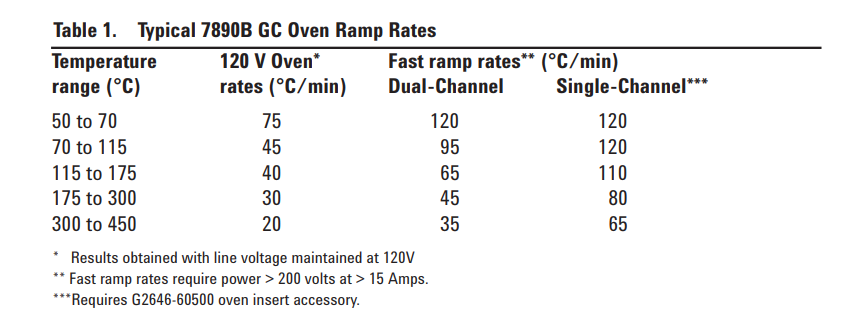
\includegraphics[width=0.8\textwidth]{Figures/7890B.png}
	\decoRule
\caption[A temperature-rate table from the Agilent7890B data sheet]{The temperature-rate table from the Agilent 7890B chromatograph data sheet\autocite{7890B}. }
\label{fig:RampRate7890B}
\end{figure}

The low ramp rate of conventional air baths are cause by three factors:

\begin{itemize}
	\item The low heat capacity of air
	\item The poor thermal conductivity of air
	\item The mass of the oven that needs to be heated. 
\end{itemize}

There is very little that can be done about these matters. In theory it would be
possible to switch oven gas to hydrogen for higher thermal conductivity, and
construct a low-mass oven using, say, advanced resins for construction, but this
would probably involve significant safety and cost issues. What is required is a
complete redesign of the heating principle.

\subsection{Resistive heating}

Fortunately the heating rate problem has a technologically simple solution,
\textit{resistive heating}. When a constant electric field is applied to a
metal, the free electrons in the metal will be accelerated by the electric
field. But the electrons are within the crystal lattice of the metal, and the
mean free path is very short. The electrons will therefore collide with atoms in
the crystal lattice, scattering inelastically. The energy lost in the inelastic
collisions will increase the vibrating frequency of atoms, and this energy will
appear as heat. The number of electrons and their average (drift) speed will
determine the current ($I$), and the electric field is best described by the
applied voltage ($V$). The current $I$ is proportional to the applied voltage,
and the ratio $\frac{V}{I}$ defines the proportionality constant $R$, called the
resistance, which is a function of conductor material and dimensions. The total
power dissipated to heat ($P$) is given by the $P=IV$ or, equivalently, $P=I^2R$
or $P=\frac{R}{V^2}$.

(Alternative methods of heating by electromagnetic fields are \textit{inductive
heating} and \textit{dielectric heating}.)

The rate at which the piece of metal heats up depends on the power dissipated,
the mass of the metal, and its heat capacity. Applying a voltage \(V\) to a
metal element in close proximity to the column will heat the metal, and
therefore the column in contact with it. If the volume of the metal is small
enough, and the current high enough, the temperature of the metal element will
increase, and with it the temperature of the column. By suitable manipulation of
\(V\) then, the temperature of the column can then be changed at any desirable
rate.

This technology has been reviewed \autocite{Wang2012,Jacobs2013}, and a few
technologies for resistive heating of capillary columns have emerged:

\begin{itemize}
  \item Direct heating of a metal column or a columns coated with metal layers
  \item Collinear heating
  \item Coaxial heating
\end{itemize}

The first SFC×GC work done \autocite{Venter2004} used a directly heated metal
column. While this approach proved the concept, experience showed two
shortcomings. Firstly, metallic columns are usually designed with specific
high-temperature applications in mind. This means that metal columns are not
available with all the stationary phases available in fused-silica columns.
Secondly, it was harder than expected to control the temperature accurately. The
temperature was determined by a thermocouple glued to the column, which was
sensitive to local variations.

Agilent\texttrademark{} supplies a `low thermal mass' column, which includes
collinear heating wire and a collinear sensing element bundled with a short
silica column. This approach requires that the collinear heating element be
wrapped in close contact with the column.

For the work presented in this thesis, we used a coaxial heater. This heater is
in the form of a thin-walled stainless steel tube that carries the electric
current. The column is threaded inside the stainless steel tube, so that it is
in close contact with the heater, giving reliable heat transfer. The metal tube
is simultaneously used as a sensing element that reports the average temperature
of the tube, and thereby the temperature of the column.

\begin{figure}[htbp]
	\centering
	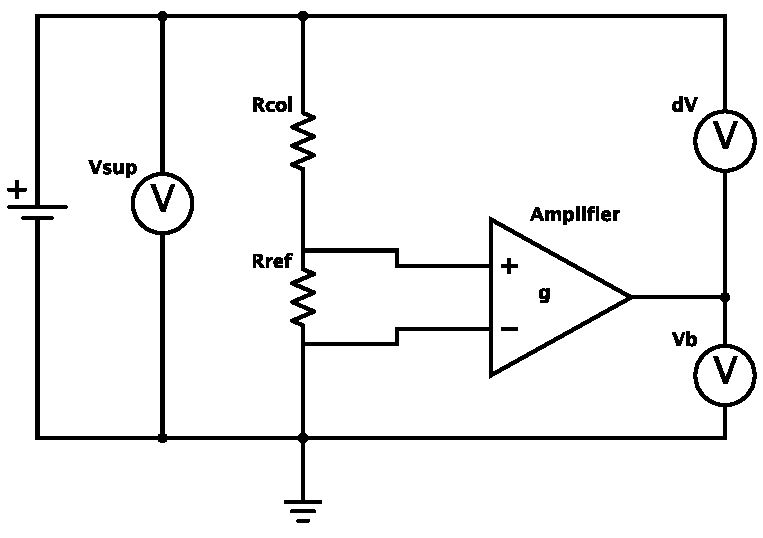
\includegraphics[width=0.8\textwidth]{Figures/Column-Heater.pdf}
	\decoRule
	\caption[Coaxial heater resistance heater]{\label{fig:HeaterDiagram}Electric circuit diagram of the coaxial heater.}
\end{figure}

The electrical resistance of a conductor is determined by its shape, the
material it is made of, and the temperature of that material. In a conductor of
given shape and dimensions, therefore, a knowledge of the resistance implies a
knowledge of the temperature. By following changes in the resistance, one can
determine changes in the resistance, and by comparing resistance at certain
temperatures with known temperatures, one can get a calibrated temperature from
a given resistance.

The circuit is supplied by a voltage $V_{sup}$, in general an unknown value.
$V_{col}$ and $V_{ref}$ represents the voltage drop over the respective
resistors.

Because the current $I$ through the circuit is the same for both $R_{col}$ and
$R_{ref}$, it is true that $\frac{R_{col}}{V_{col}}=\frac{R_{ref}}{V_{ref}}$,
and therefore \begin{equation}R_{col} = R_{ref}\frac{V_{col}}{V_{ref}}
\end{equation}

The voltage drop across $R_{ref}$ is small, and therefore it is amplified by the
amplifier with gain $g$, so that $V_b = gV_{ref}$. $V_b$ is measured, as is
$dV$, the potential difference between the supply and the amplifier output.

$V_{sup} = V_{col} + V_{ref}$ 

$V_{sup}=dV + V_b$

$V_{col} + V_{ref} = dV + V_b$

$V_{col} + V_{ref} = dV + gV_{ref}$

$V_{col} = dV + gV_{ref} - V_{ref} $

$V_{col} = dV + V_{ref}(g - 1)$

$\frac{\displaystyle V_{col}}{\displaystyle gV_{ref}} = dV/gV_{ref} + V_{ref}(g-1)/gV_{ref}$

$\frac{\displaystyle V_{col}}{\displaystyle V_{ref}} = gdV/gV_{ref} + gV_{ref}(g-1)/gV_{ref}$

$\frac{\displaystyle V_{col}}{\displaystyle V_{ref}} = gdV/V_b + (g-1)$

This proves that $\frac{\displaystyle V_{col}}{\displaystyle V_{ref}}$ is a
linear function of $dV/V_b$. A quick check for correctness of the expression:
for a unity-gain amplifier $g = 1$, and $\frac{\displaystyle
V_{col}}{\displaystyle V_{ref}} = dV/V_b$.


\subsection{Assumptions}

The assumption is that the temperature is a function of the resistance of the
column, or $T = f(R_{col})$. Because $R_{col}=m(^{dV}/_{V_b}) + c$, we can say
that $T = f^{-1}(^{dV}/_{V_b})$. Through a calibration procedure $f^{-1}$ can be
approximated by a polynomial or lookup table.

\subsection{Heating control and temperature programming}

\subsection{Temperature uniformity}
\label{sec:Uniformity}

It is highly desirable that the coaxial heater should give uniform heating.
There is no guarantee that this will be the case. We did not analyse the problem
theoretically, but the following factors need to be considered:

\subsubsection{Resistivity's dependence on temperature}

The  resistance of a metal increases with temperature. This means that if one
section of the coaxial heater should get hotter than the rest, it's resistance
will increase. If the current were to remain constant, more power would be
dissipated in this section (\(P=I^2R\)). If more power is dissipated, the
temperature will increase, leading to a higher resistivity, leading to higher
power dissipation, leading to a higher temperature, in a runaway cycle. If the
supply voltage was held constant a higher resistance in one section would mean a
lower current overall, but still a higher power dissipation in the section with higher temperature. 

\subsubsection{Thermal conduction}

Each section of the coaxial heater is in thermal contact with its neighbours. If
it were to get hotter, the heat will flow from the hotter section to the cooler
neighbouring sections. This will tend to even out any temperature differences.

\subsubsection{Radiation}

An object radiates heat, which can be approximated by the Stefan-Boltzman law:

\[P=A \epsilon \sigma T^4\]

where A is the surface area of the object, \(\epsilon\) is the
\textit{emissivity} of the surface, \(\sigma\) is the Stefan-Boltzman constant,
and \(T\) is the absolute temperature of the object. 

If a section of the coaxial heater were to become hotter than the other
sections, it would therefore radiate more heat. The increased power dissipation
by the higher resistance will therefore be partially offset by a higher
radiation. This will tend to moderate moderate temperature differences.

\subsubsection{Thermal imaging}

The combination of resistivity's temperature dependence, thermal conduction and
radiation can probably be modelled, but such an endeavour would fall outside the
scope of the project. Experience had not lead us to expect any significant
temperature non-uniformity, but we had the opportunity to get empirical
confirmation.

\textit{Thermal imaging} is the process by which infrared radiation from objects
can be captured in a photographic process. At near-ambient temperatures objects
emit copious amounts of infrared radiation, and higher the temperature, the more
is emitted. Using specialized optics and sensors allows the capture of that
radiation in a camera, which can produce an image of a scene that shows objects
based on their surface temperature. The technological capability of thermal
imaging has improved markedly over the past years

Using a FLIR{\texttrademark} T660 thermal imaging camera we obtained a video of
the coaxial heater executing a temperature ramp. This camera uses a \num{640 x 480}
focal plane uncooled bolometer array as a detector, which is sensitive to
radiation in the range \SI{7.5}{\micro\metre} to \SI{14}{\micro\metre}.
Figure \ref{fig:ThermalImageSetup} shows the setup used to record the thermal
video.

\begin{figure}
	\centering
	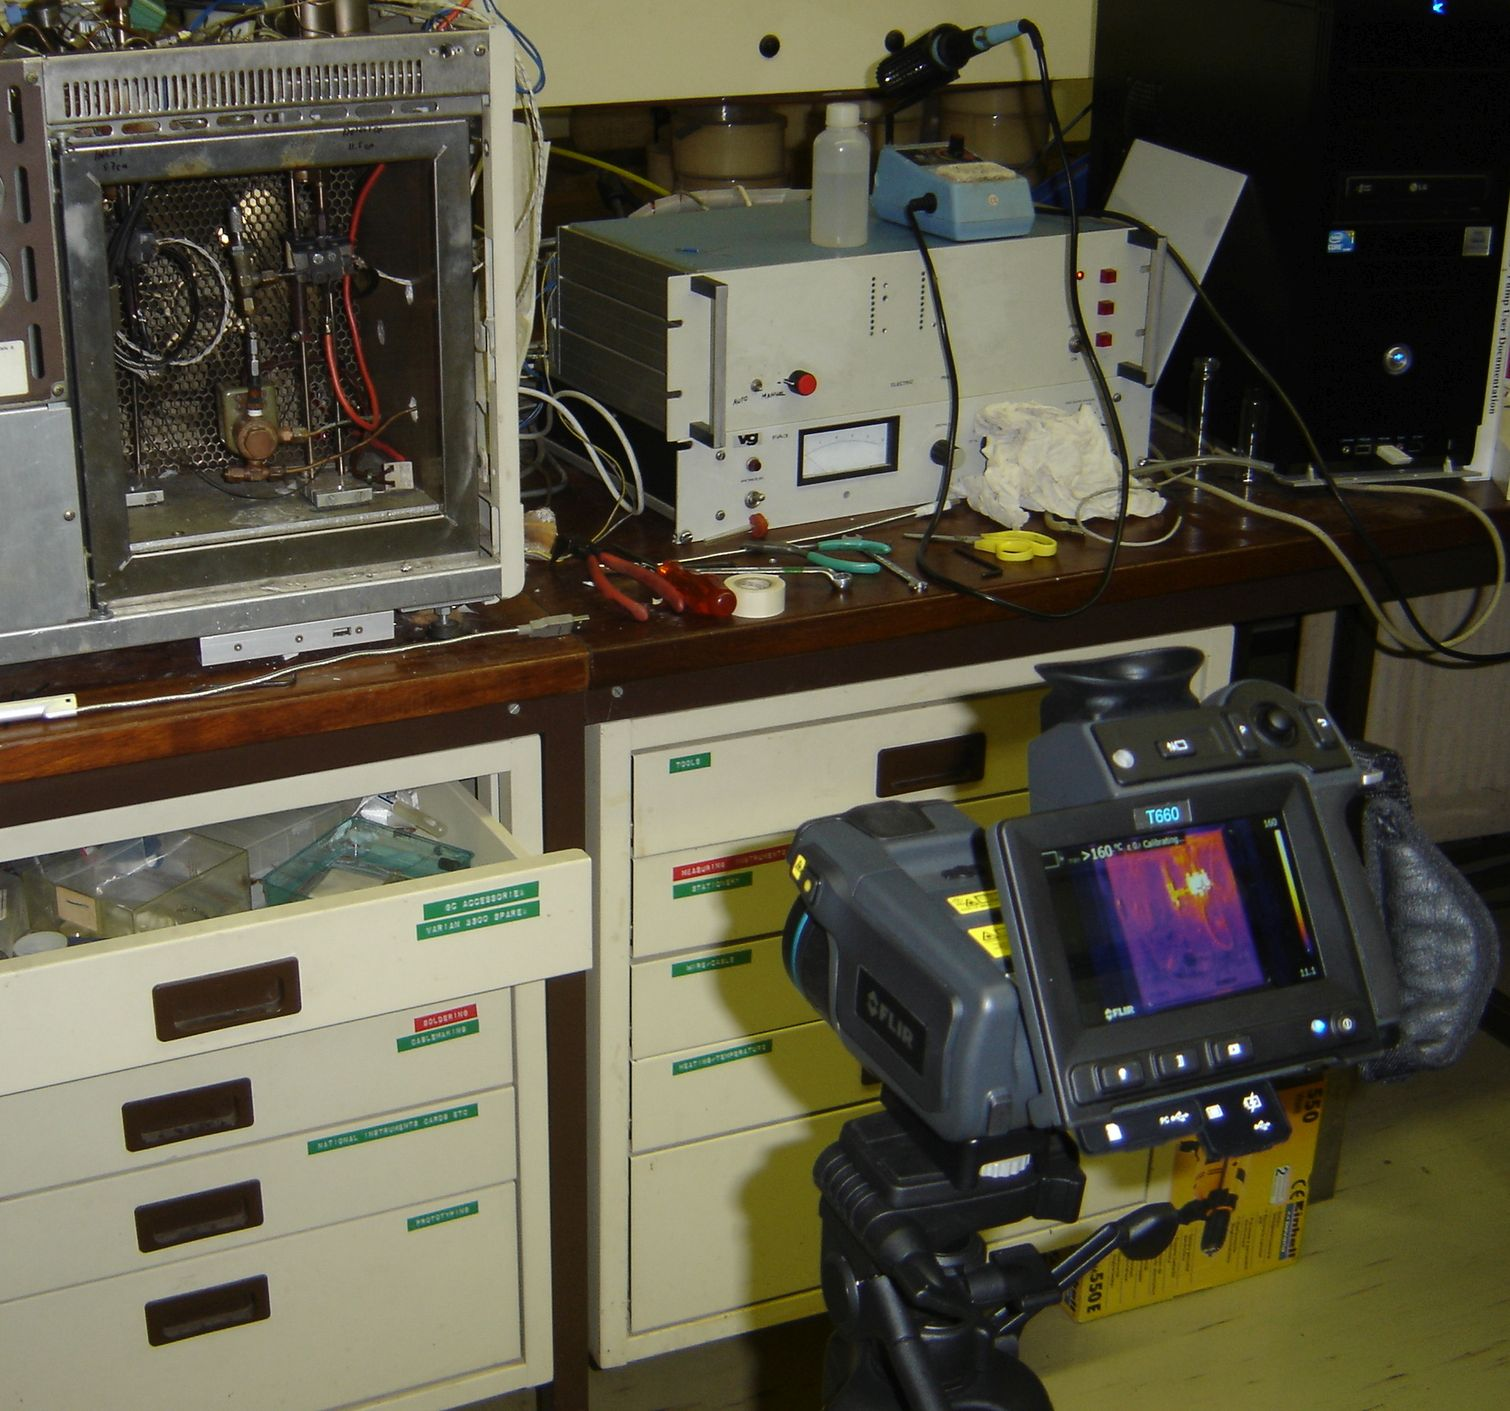
\includegraphics[width=0.8\textwidth]{Figures/ThermalImageSetup}
	\decoRule
	
\caption[A photograph of the setup used to record the thermal video]{This
photograph shows the setup used to record the termal video.}
	
	\label{fig:ThermalImageSetup}
\end{figure}

Figure \ref{fig:ThermalImage} is a frame from the video, analysed to give
estimates of the temperatures on spots on the coaxial heater. The maximum
temperature difference between any two points is \SI{17.5}{\celsius}, and there
are no marked gradients.

\begin{figure}
	\centering
	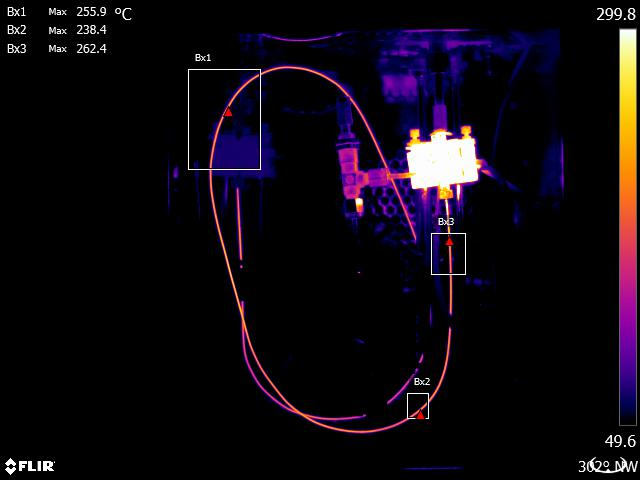
\includegraphics[width=0.8\textwidth]{./Figures/ThermalImage}
	\decoRule
	
\caption[A thermograph of the coaxial heater at temperature]{A thermograph of
the coaxial heater at high temperature. It shows that there are no runaway hot
spots.}
	
	\label{fig:ThermalImage}
\end{figure}

This examination of the uniformity of the coaxial heater put to rest any fears
that unexpected temperature gradients would interfere with the fast gas
chromatography.

\subsection{Temperature calibration}

When doing temperature-programmed gas chromatography it is desirable to have an
absolute measurement of the temperatures. This makes it possible to translate
methods between instruments. It was therefore necessary to attempt to calibrate
the coaxial heater.

The problems of measuring a temperature inside a tube with a bore of
\SI{0.8}{\milli\metre} are not trivial.

The following technologies exists to measure temperatures:
\begin{itemize}
	\item Liquid-in-glass thermometers
	\item Sealed liquid or gas sensing instruments and bimetallic sensors.
	\item Electrical resistance temperature measurement using metallic sensors
	\item Thermistors and semiconductors
	\item Thermoelectric temperature measurement
	\item Disappearing filament optical pyrometer
	\item Photoelectrical optical pyrometers
	\item Total radiation pyrometers.
\end{itemize}

Liquid-in-glass thermometry would not be applicable because of the size of the
devices, and because they don't give a desirable electrical signal. 

In recent years the technology for measuring temperature by radiant energy
methods have improved markedly and has become affordable, in the form of thermal
cameras. However, at lower temperatures the accuracy of the recorded temperature
depends heavily on the emissivity of the measured material. Thermal imaging will
also only measure the outside wall surface temperature of the heater, and not
the temperature of the inside of the coaxial heater. So, while thermal imaging
settled questions about heater uniformity (Section \ref{sec:Uniformity}), it was
not considered ready to serve as a calibration standard. 

This leaves us with resistance temperature measurement with metallic sensors,
thermistors and semiconductors, and thermoelectric temperature measurement.

Electrical resistance measurement using metallic sensors is quite feasible, if a
sensing element of the appropriate dimensions was commercially available. Additionally,
because long, thin wires would be needed to connect the sensing element to the
electronics, correction for the resistance of those conductors would have to be made.

Thermistor and semiconductor devices could, in principle, be made small enough
for the job, but commercially available devices come in 'packages' are too
large. Besides, the operating temperature range is a bit extreme for
semiconductors that generally have an upper operating temperature limit of
\SI{125}{\celsius}.

Thermoelectric temperature measurement then remains. In particular, the
\textit{Seebeck effect} was exploited, which is the observation that a
temperature gradient imposed on a conductor will generate an electrical
potential along the gradient. Therefore, a circuit of two dissimilar metallic
conductors will generate a voltage when there is a temperature gradient along
the conductors. The voltage generated is a function of the temperature
difference between the junctions of the two metals. Such a pair of dissimilar
conductors used to generate a voltage is known as a \textit{thermocouple}.
Thermocouples are widely used in industry for measuring temperatures, and the
technology is well established. Thermocouple wire can be purchased in varying
gauges, down to \SI{25}{\micro\metre} in diameter, and the signal processing for
thermocouple signals have been standardized.

McGee \autocite{McGee1988} states that thermocouple junctions can be made by
welding, crimping, soft soldering, hard soldering, bolting, or simply twisting
the wires together.

Because of the temperature range expected to be measured ({-}50 \si{\celsius} to
400 \si{\celsius}) the option of soft soldering does not apply, because soft
solders have a melting points around \SI{200}{\celsius}. The possibility of
corrosion and mechanical vibration suggest that twisting the wires together
will not form a reliable joint, and of course there are no sub-millimetre bolts
on the market.

This leaves welding, crimping and hard soldering. The option of crimping was not
explored, chiefly because we have no knowledge of technology or devices that can
crimp hair-fine wire. Our knowledge of crimping suggest that shows another
problem: the final crimped connection has a diameter many times the diameter of
the wire. This precludes the application of crimping in this context.

Hard soldering is usually done with high-temperature flames, and on contact the
flames will rapidly burn the fine wires. The temperatures required for hard
soldering is still lower than the melting point of the wires, so that hard
soldering is not excluded, but we did not have the knowledge or the technology
to solve the associated problems.

Welding was found to be an accessible technology for forming small, reliable
joints in fine fine thermocouple wire.

\subsection{Thermocouple Welding}

Welding is the process of joining two metal parts by melting a portion of each
part, allowing the molten metal first to mix, and then solidify. This creates a
permanent joint between the two metals. Welding is widely practised as an
industrial process.

Various sources of heating can be used, and we decided to use electricity. A
\SI{24}{\volt} direct current, adjustable bench power supply was used. The two
wires of the thermocouple was twisted together, and the twisted pair was
connected to one pole of the power supply. A carbon electrode was connected to
the other pole. The carbon electrode was carefully brought closer to the
thermocouple pair until a spark jumped across the air gap. When the spark turned
into an arc, the heat of the arc melted the thermocouple. The molten metal would
then contract into a spherical globule, which grew as the arc added more heat.
As more of the metal of the wire melted, the globule would move away from the
carbon electrode, until the gap became too large to sustain the arc. The current
would then stop, and leaving a spherical welded at the end of the wires. The
process could be repeated as often as necessary to obtain a bead of the desired
size. The steps of the process is shown in Figure \ref{fig:WeldingSteps} It is
worth noting that it is absolutely necessary to form an arc: if the carbon
electrode happened to touch the wire so that a current flowed directly from the
wire to the carbon electrode the wire would rapidly heat up over its length, and
melt. It is also interesting to note that it seemed necessary to have a roughly
broken carbon electrode surface: a polished surface would not generate an arc,
or even make electrical contact with the wires. This might be because the
graphite used for the electrode was formulated for use in pencils.

\begin{figure}
	\centering
	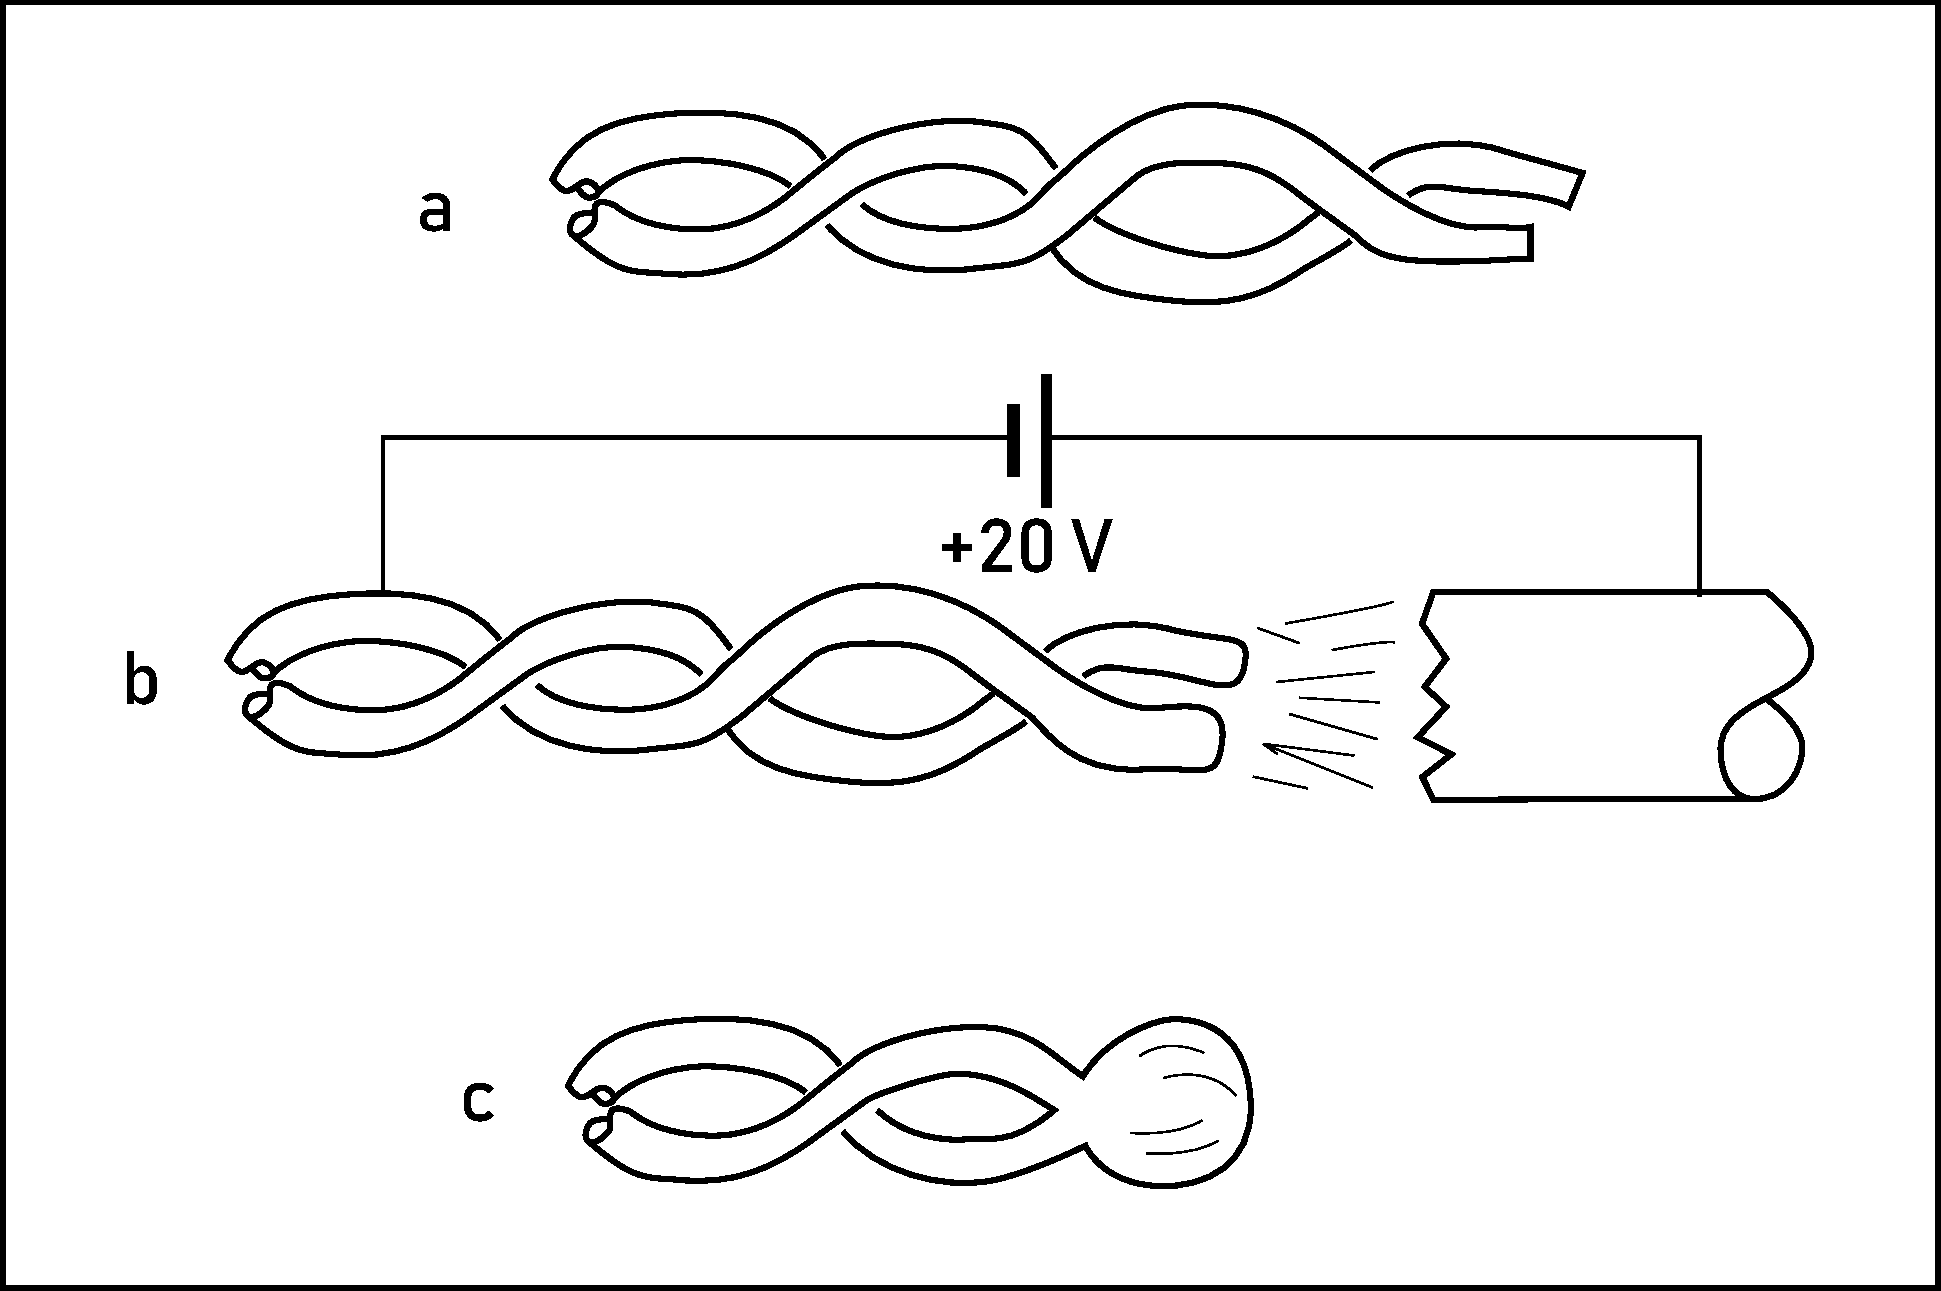
\includegraphics[width=0.8\textwidth]{Figures/TCWelding}
	\decoRule

\caption[Welding process schematic]{The process of welding fine wires to make
thermocouples (a) Wires twisted together (b) Electric arc heating up the wires
(c) Wires welded with a well-formed bead. }

\label{fig:WeldingSteps}
\end{figure}


\begin{figure}
	\centering
	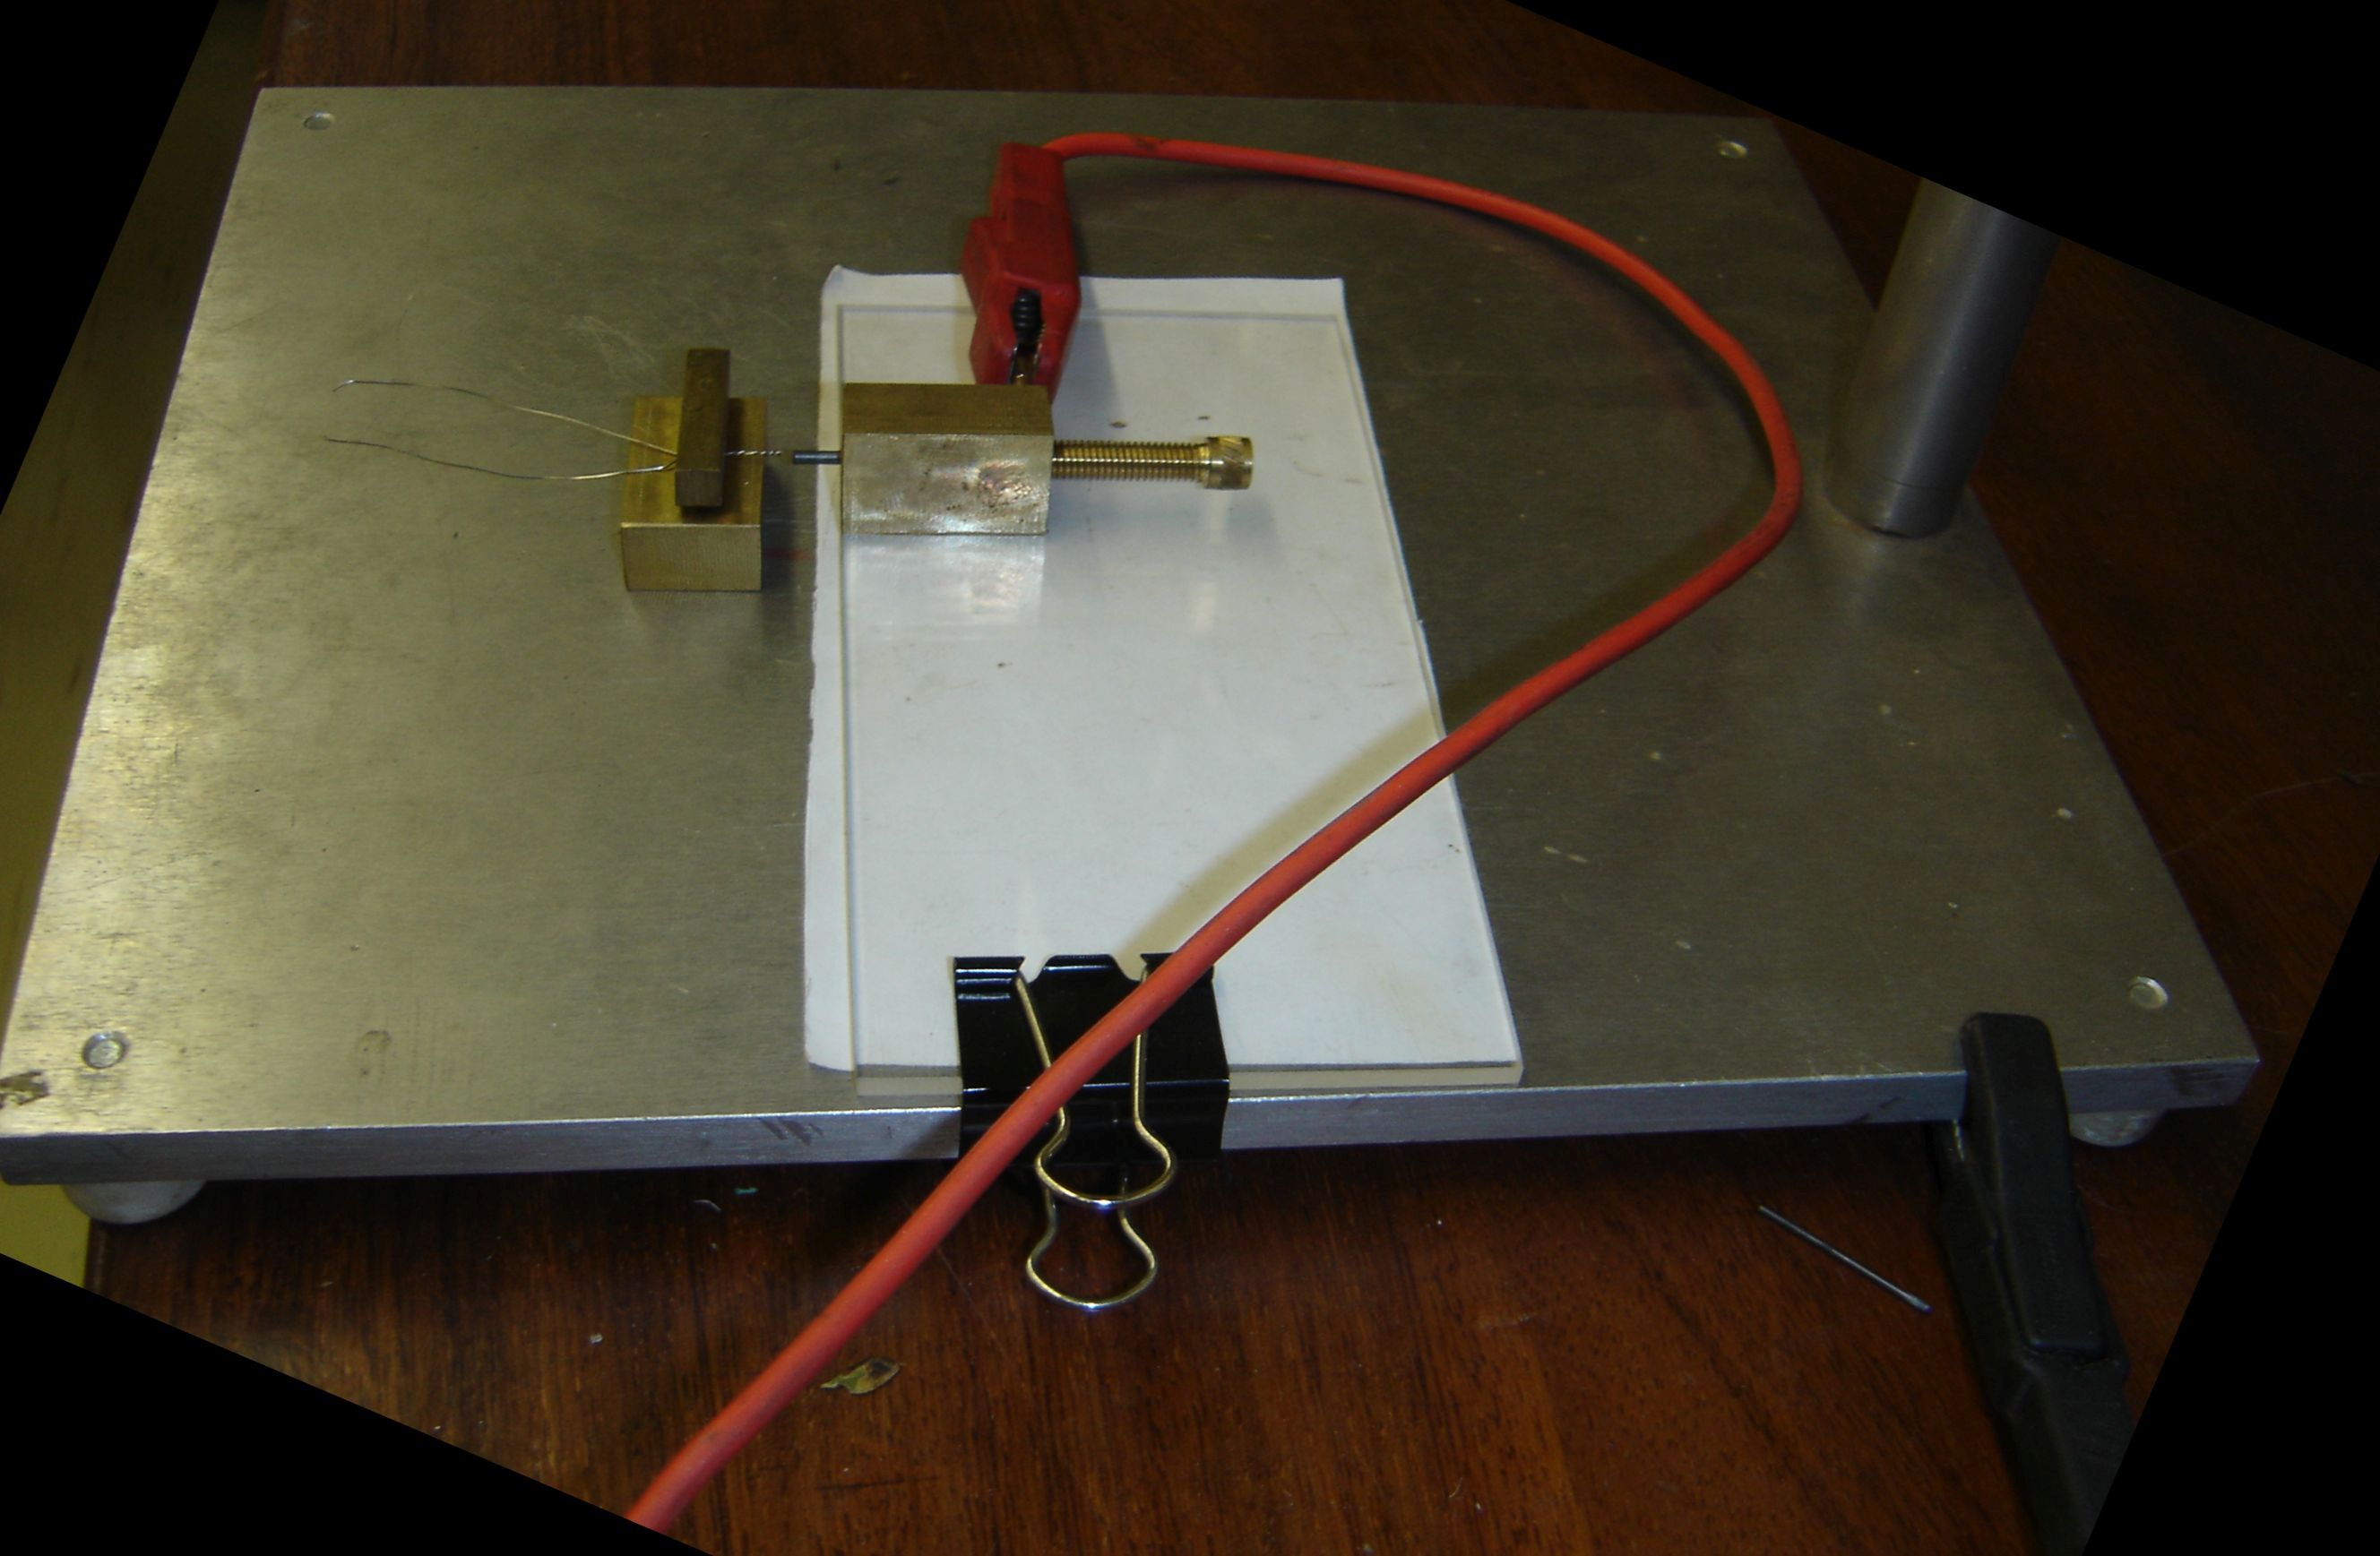
\includegraphics[width=0.8\textwidth]{Figures/Welder2.jpg}
	\decoRule

\caption[Fine-wire welder]{A view of the fine-wire thermocouple welder. The wire
shown is much thicker than that actually used. It is shown clamped between the
clamping bar and the clamping weight. A thin sheet of acrylic serves to isolate
the positive electrode from the negative base. The carbon electrode can be
advanced towards the thermocouple twist using the screw. The black clamp at the
bottom right-hand corner attached to the base plate and the red clamp attached
to the screw housing provide a potential difference of approximately \SI{20}{V}
between the carbon electrode and the thermocouple.}


\label{fig:FineWireWelder}
\end{figure}



\begin{figure}
	\centering
	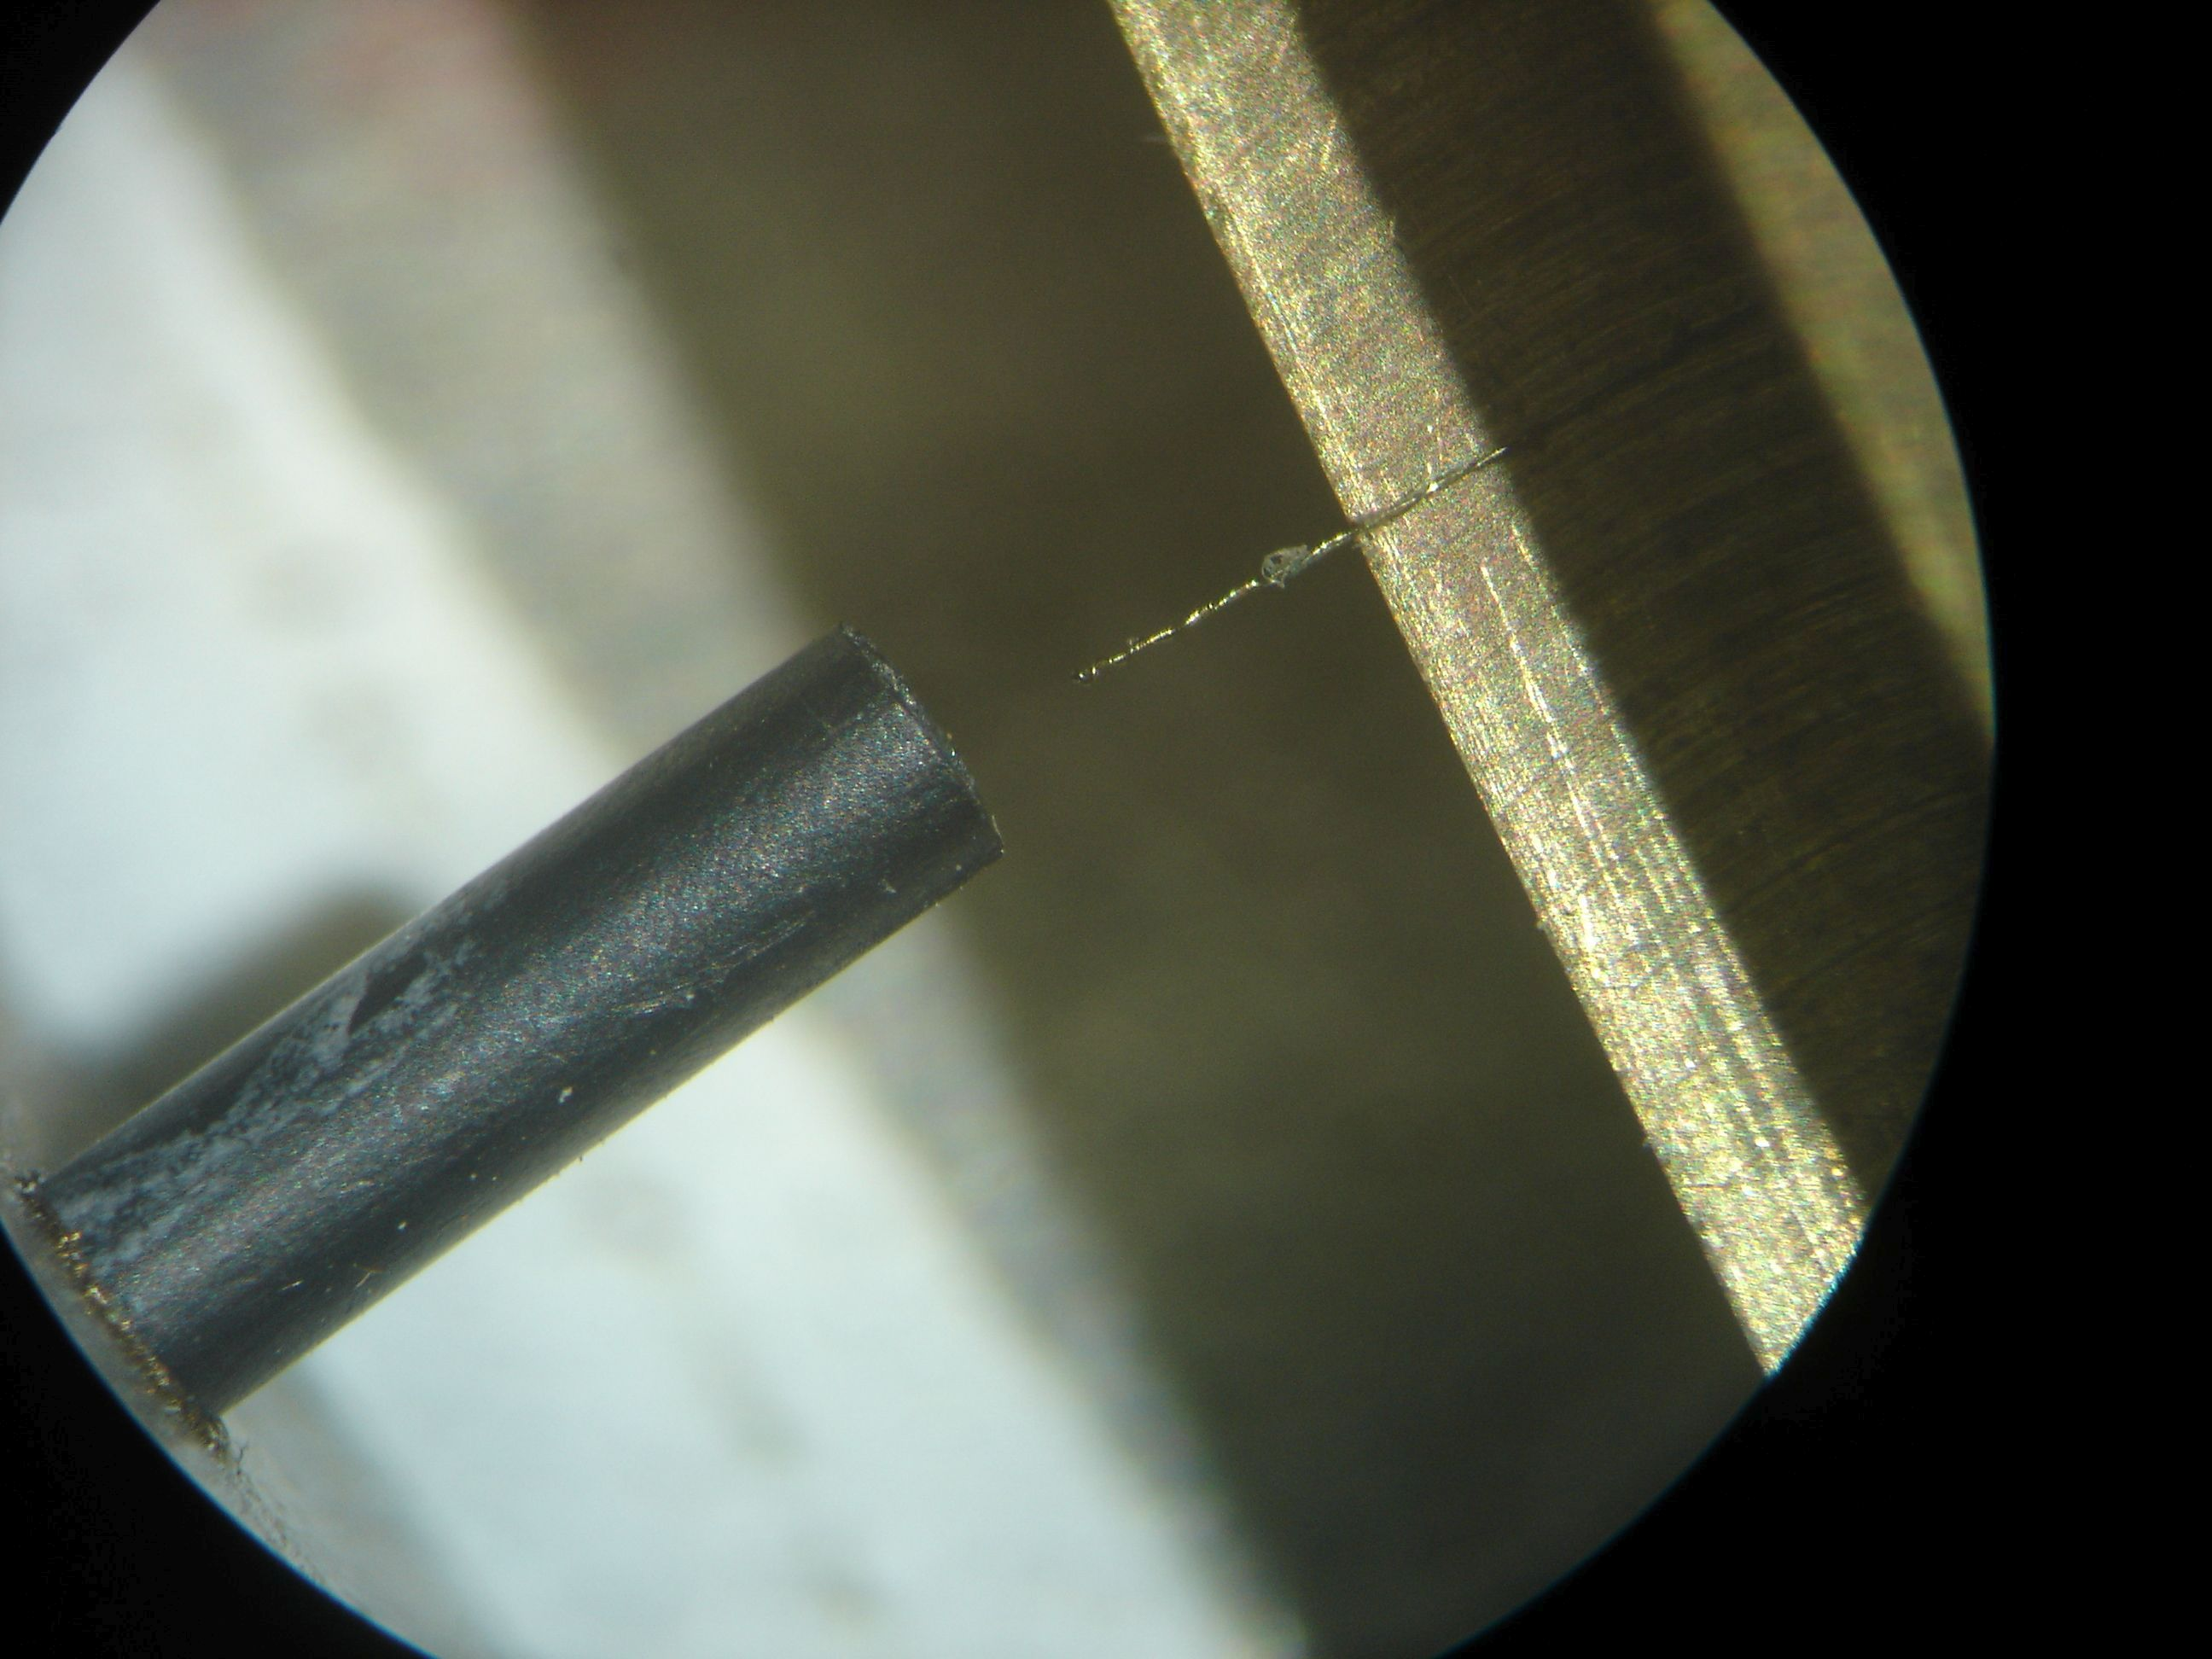
\includegraphics[width=0.8\textwidth]{./Figures/WelderMicro.jpg}
	\decoRule
	
\caption[A microphoto of a thermocouple twist ready to be welded.]{A microphoto
of a twisted wire ready to be welded. The black carbon electrode is
\SI{2}{\milli\metre} in diameter.}
	
	\label{fig:TCWeldMicro}
\end{figure}

\subsection{Termocouple probe construction}

To measure the temperature inside the coaxial heater required the thermocouple
used for the measurement had to be inserted into the coaxial heater. For this we
used fused silica capillaries with an inside diameter of \SI{0.25}{\milli\metre}
and an outside diameter of \SI{0.4}{\milli\metre}. These were easily obtained in
the form of worn-out chromatographic columns. A thinner capillary was used to
draw the wires into the probe capillary, in a process described in Figure
\ref{fig:FineWireThermocouple}

\begin{figure}
	\centering
	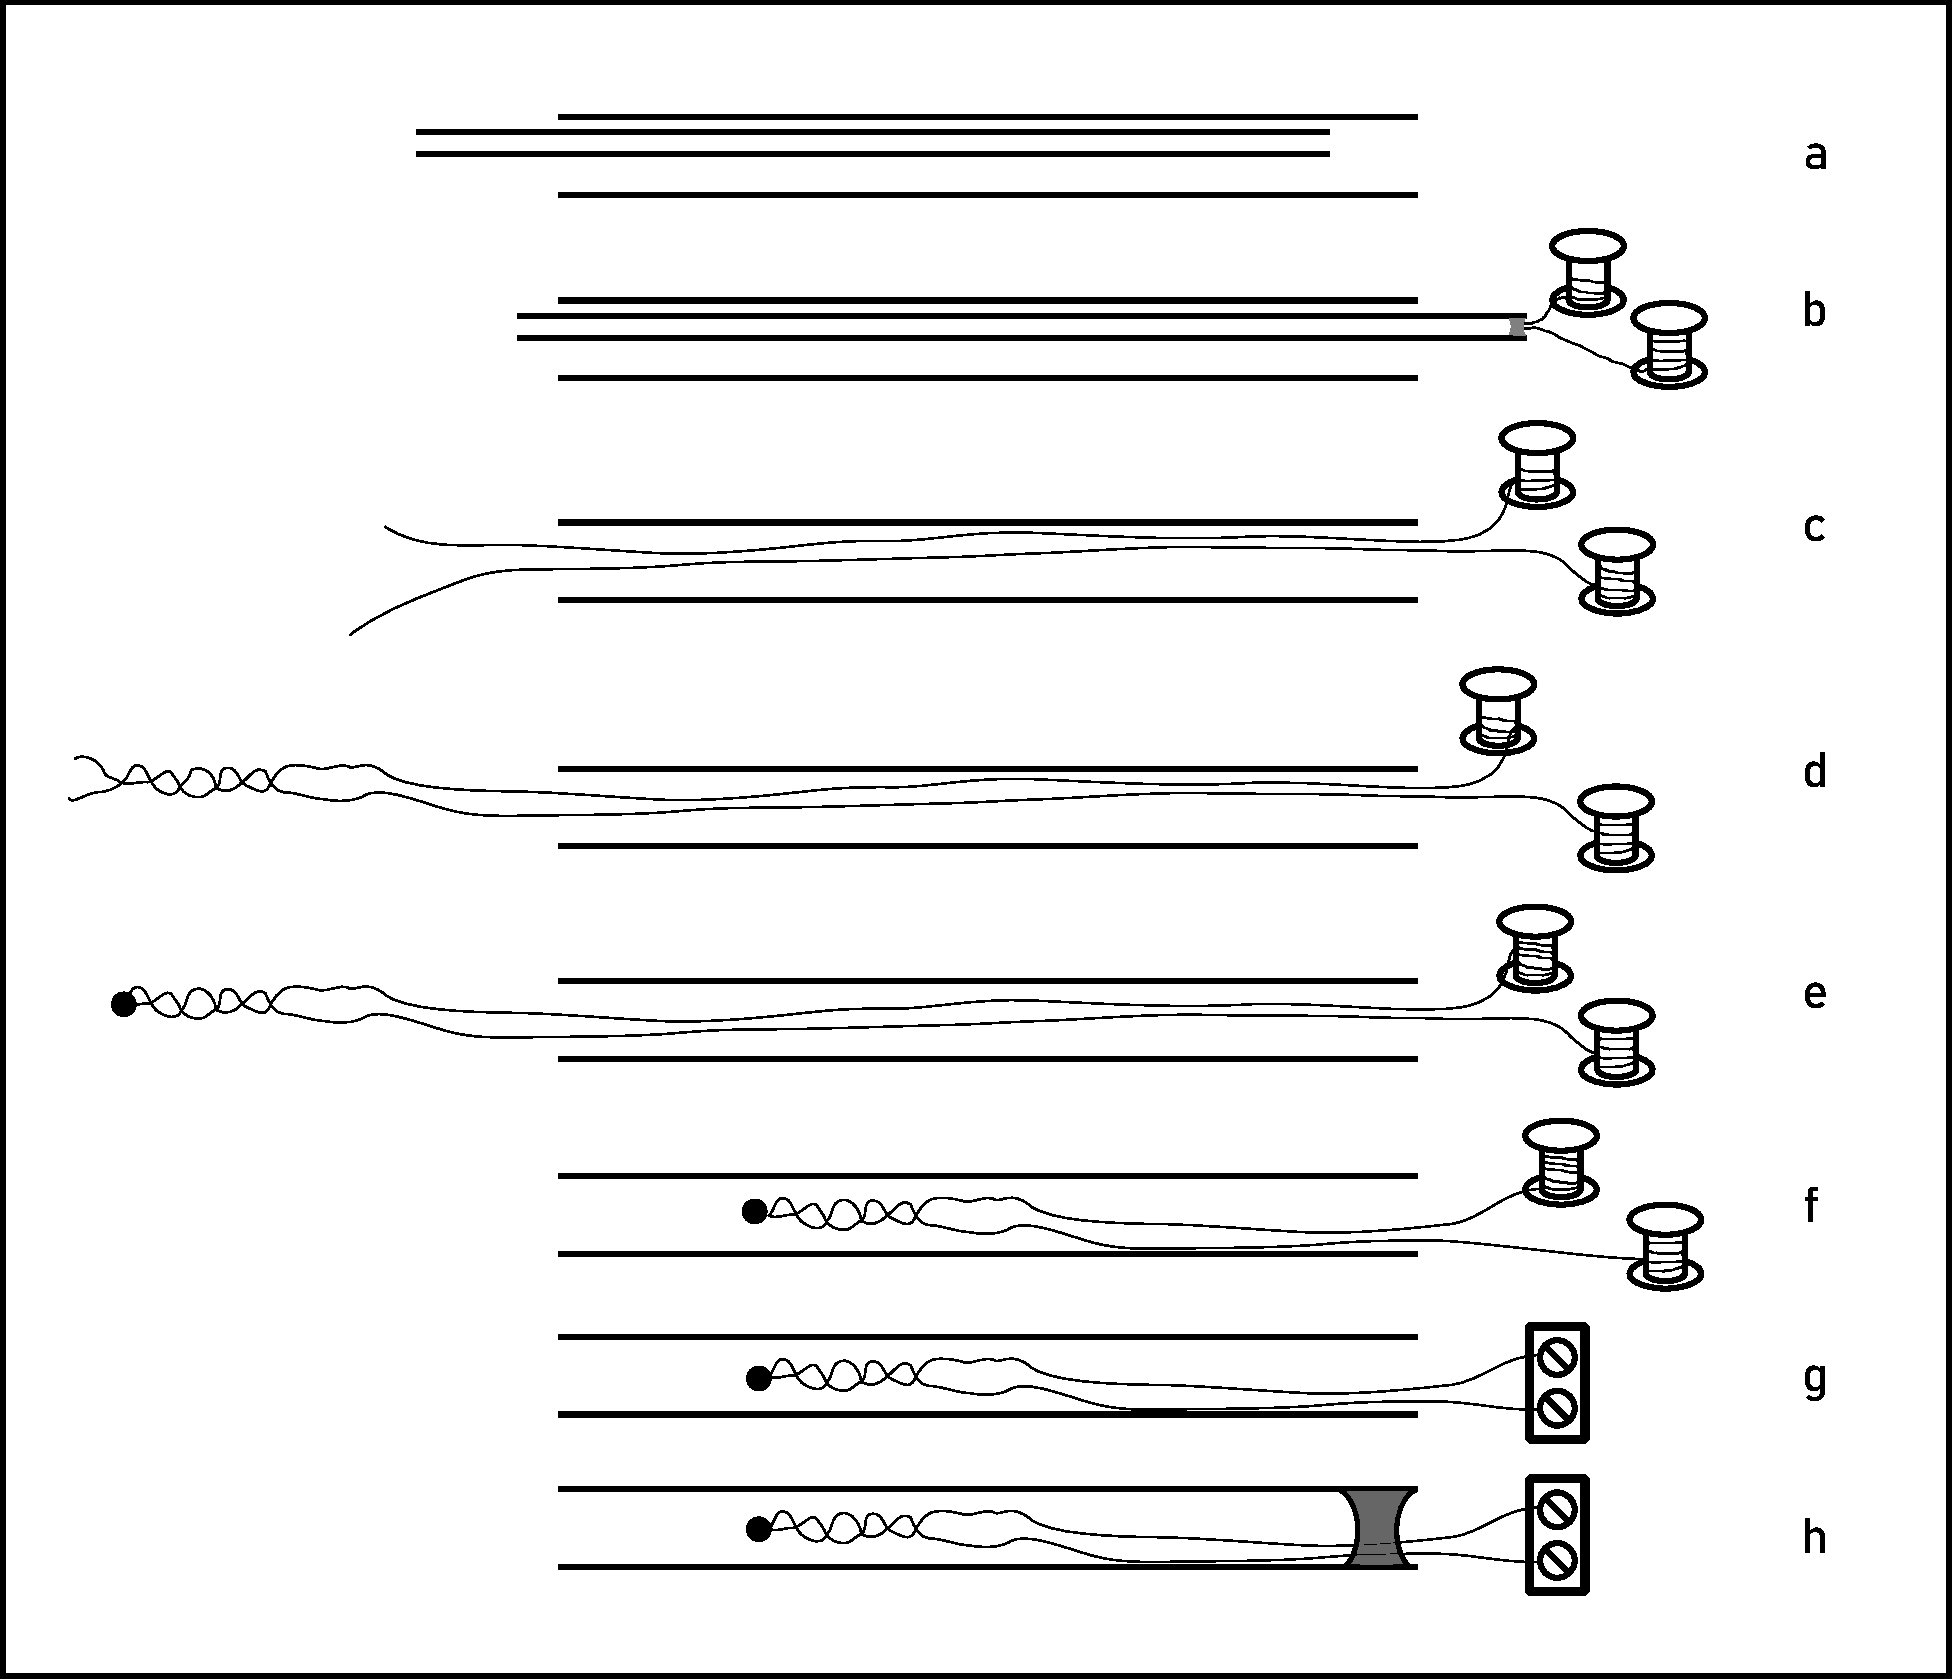
\includegraphics[width=0.8\textwidth]{./Figures/FineWireThermocouple.pdf}
	\decoRule
	
\caption[A cartoon explaining how to construct a long, thin thermocouple
probe.]{(a) A thin capillary is threaded inside a thicker one (b) The ends of a
pair of thermocouple wires are fitted inside the end of the thin capillary. (c)
The wires are pulled through the thick capillary using the thin capillary. (d)
The ends of the wires are twisted together, creating a mutual mechanical anchor.
(e) The ends of the wires are welded together. (f) The wires are pulled back
into the thick capillary, locating the junction at the desired position in the
capillary. (g) The wires are trimmed and connected to a terminal block. (h) A
drop of cyanoacrylate adhesive is used to anchor the wires permanently in the
capillary. }
	
	\label{fig:FineWireThermocouple}
\end{figure}

\subsection{Calibration procedure}



\subsection{Cold spots}
\label{sec:ColdSpots}

For fastest temperature programming the heating element should be as light as
possible, and carry the largest necessary current. In practice, the current
doing the heating must be carried to the coaxial heater using a conductor. To
prevent the feed conductor from heating up it must have a low resistance, and
this low resistance is achieved by making the conductor as 'thick' or as 'heavy'
as necessary, meaning that it should be constructed of a material with a high
mass per unit length.

Good electrical metallic conductors are invariably also good thermal conductors,
and therefore the area around the junction of the feed conductor to the coaxial
heater will always have a lower temperature than the nominal temperature of the
heater. In capillary GC this is undesirable: a cold spot in a column can wreak
havoc with retention times and peak shapes.

Conversely, if an attempt is made to reduce the contact area between the feed
conductor and the thin material of the coaxial heater, a hot spot might develop,
which could burn a hole in the coaxial heater tube or damage the column.

The electrical connection between the feed conductor and the coaxial heater was
therefore designed in the form of an externally heated block. This block was
kept at a higher temperature than the highest expected temperature of the
chromatographic temperature program. This prevented the formation of cold spots
in the coaxial heater, which might lead to cold spots in the column, while still
offering a large contact area so that hot spots do not develop.

Each end of the coaxial heater therefore ended in a heated block. Each block was
heated by four \SI{100}{\watt} Hotset\texttrademark{}electrical cartridge
heaters, with dimensions of \SI{6.5 x 40}{\milli\metre}. The cartridge heaters
were switched on and off by solid state relays controlled from the computer. The
temperature of the block was monitored through a thermocouple and the amount of
power to the heaters was controlled by pulse width modulation (PWM) implemented
in software. \todo
 
\subsection{Cold column}

In a cold stationary phase the retention factor \(k'\) is very high. This means
that the analytes migrate slowly relative to the mobile phase. The lower the
temperature, the higher \(k'\) becomes, so that for very low temperatures the
migration of the analyte becomes negligible. In effect, the analytes are
'trapped'. This trapping, also called \textit{cryotrapping} or
\textit{cryofocusing} is useful in various aspects of gas chromatography, such
as two-stage thermal desorption or thermal modulation in GC×GC. 

\todo{Potgieter PTV trap}

In the SFC×GC instrument described here, cryotrapping was used as the second
stage to a two-stage modulator. (The stop valve described in Section
\ref{sec:stopflow} represents the first stage.) The column was cooled down to
very low temperatures, which trapped any analytes eluting from the first
dimension in a narrow band on the GC column. Once the required amount of
fraction had been collected, the flow from the first dimension would be stopped
by closing the stop valve. Then the temperature ramp of the fast GC could start.
As the coaxial heater warmed up the column the solubility of the analytes would
decrease, and the analytes would start migrating.

The first SFC×GC chromatograph cooled the column by using the cryo-cooling
function of the Varian 3300 GC. The purpose of this function is to cool the GC
column down to sub-ambient temperatures. This function is needed when analysing
very volatile compounds. In such cases the \(k'\) values at or near room
temperature are too low to provide adequate retention, and the cryo-cooling
function permits low-temperature temperature programs.

The Varian 3300 cryo-cooling function works by injecting liquid carbon dioxide
into the oven. The evaporating liquid carbon dioxide absorbs energy from the
air, which lowers the temperature of the air in the oven. A control system
controls the amount of carbon dioxide admitted and the amount of heat added
through the oven heaters, thereby keeping the oven at the required temperature.

While the cryo-cooling function can cool down an oven to cryo-trap analytes,
there are two reasons why it is not a suitable method for practical trapping in
SFC×GC. The first reason is the quantity of coolant required: doing SFC×GC runs
revealed that about \SI{15}{\kilogram} of carbon dioxide was consumed per
run. A standard cylinder of carbon dioxide contains \SI{33}{\kilogram}, which
implies that a new cylinder would be required every two runs. Such a rate of use
is much too high for the intended application of the instrument. The second
reason using the GC oven's cryo-cooling function was not suitable for SFC×GC is
that it is much too slow. Cooling the column in an air bath has the same
drawbacks of low conductivity and low heat capacity as heating it (see Section
\ref{sec:RampRates}.

A system was therefore developed by which liquid carbon dioxide is injected from
one end into the space between the column and its coaxial heater. The other end
is open to the atmosphere. When the pressure of the carbon dioxide drops from
\SI{55}{atm} to \SI{1}{atm}, the liquid starts boiling, absorbing large
quantities of heat from the surrounding column and coaxial heater, so that their
temperatures decrease rapidly. This system solves the two problems posed by the
cryo-cooling function: because the coolant is in direct contact with the parts
that need to be cooled, the cooling is rapid, and because the coolant is applied
where it is needed, only a small quantity is required.

The carbon dioxide for cooling the coaxial heater was introduced through the
same heated block that provided the electrical connection. (See Section
\ref{sec:ColdSpots}.) A T-piece design allowed the liquid carbon dioxide to be
admitted to the end of the coaxial heater, which was brazed to the block. The
column exited the block through a micro-union brazed to the block, and the
liquid carbon dioxide entered along the side of the T (Figure
\ref{fig:ManifoldDims} and Figure \ref{fig:ManifoldAssy}.  A metering valve
allowed the flow rate of the coolant to be adjusted, and a solenoid valve could
switch the flow on or off under computer control.

\begin{figure}
	\centering
	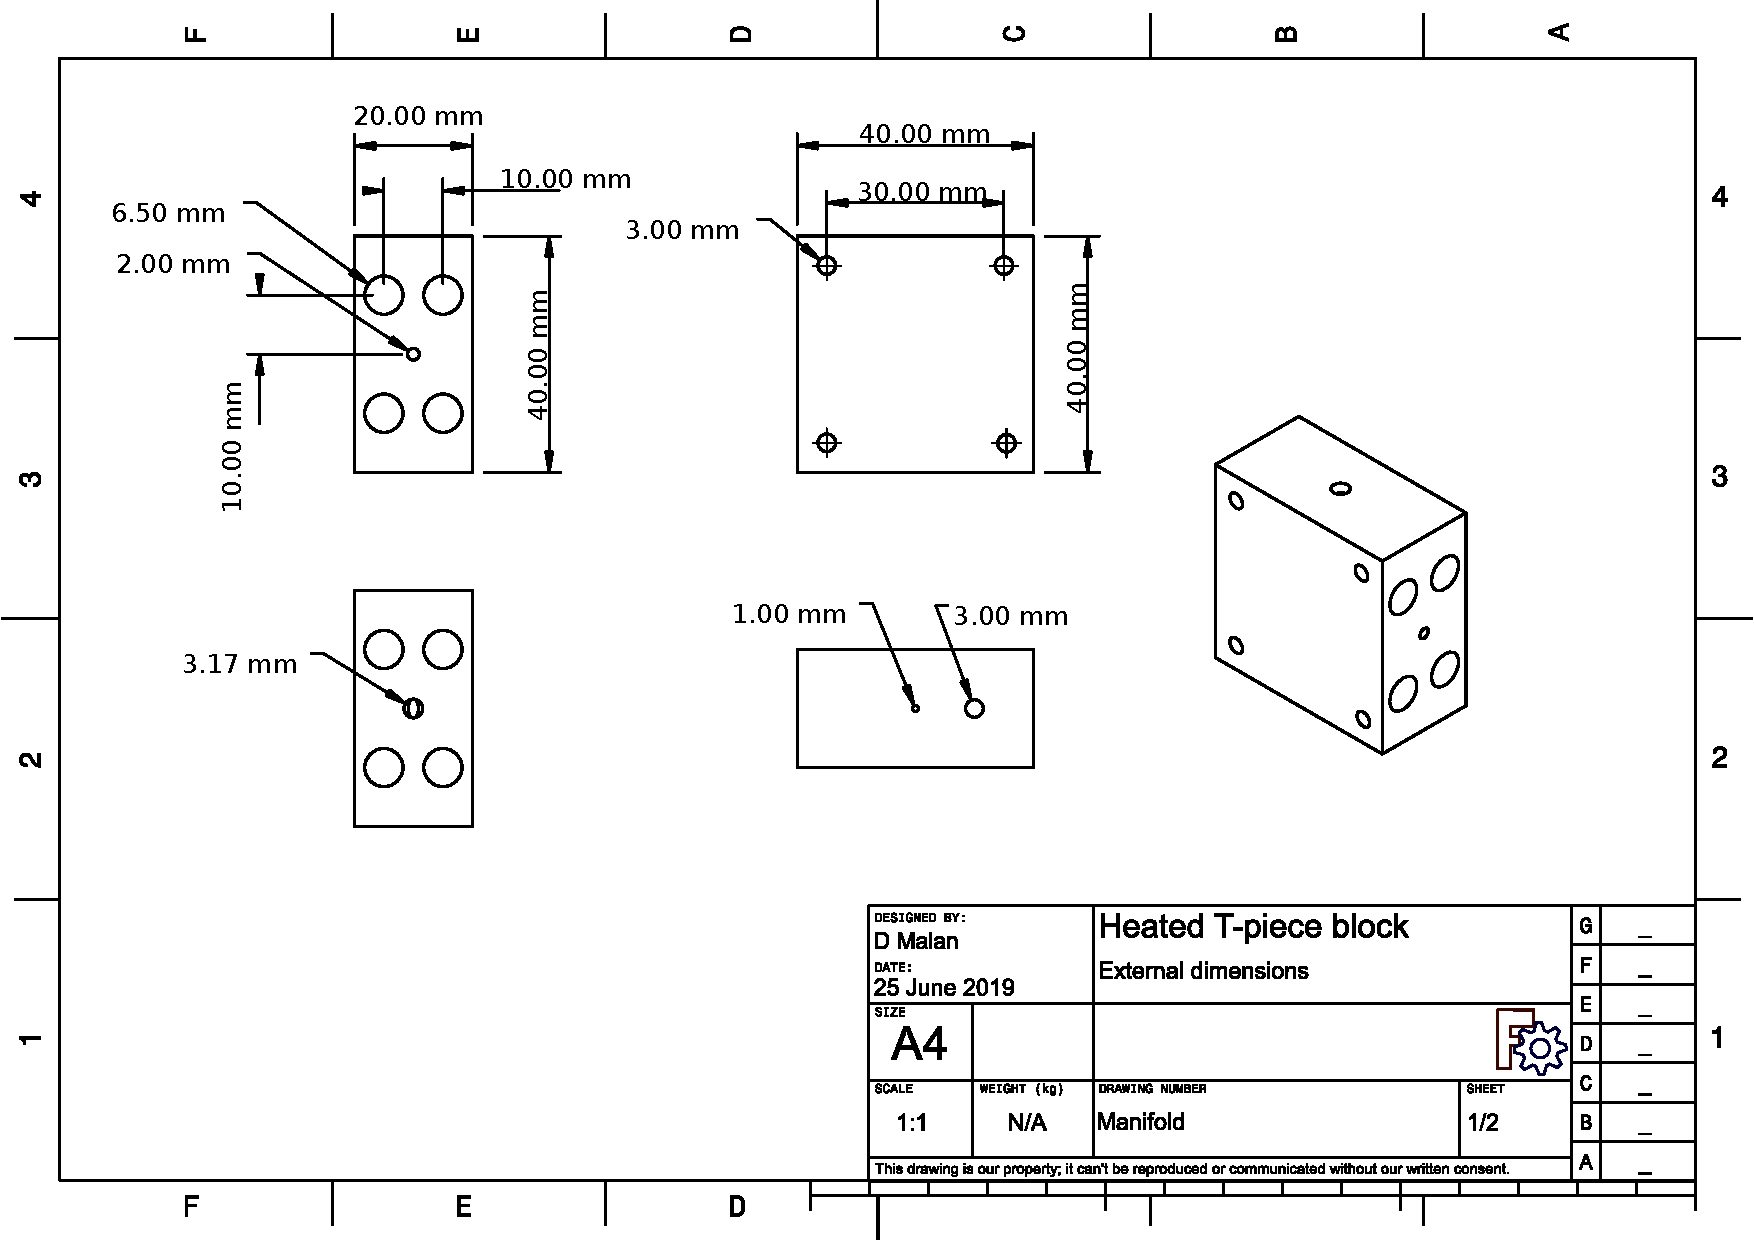
\includegraphics[angle=90, origin=c, width=0.8\textwidth]{./Figures/ManifoldDimensions.pdf}
	\decoRule
	\caption[Manifold dimensions.]{Dimensions of the heated T-piece blocks}	
	\label{fig:ManifoldDims}
\end{figure}

\begin{figure}
	\centering
	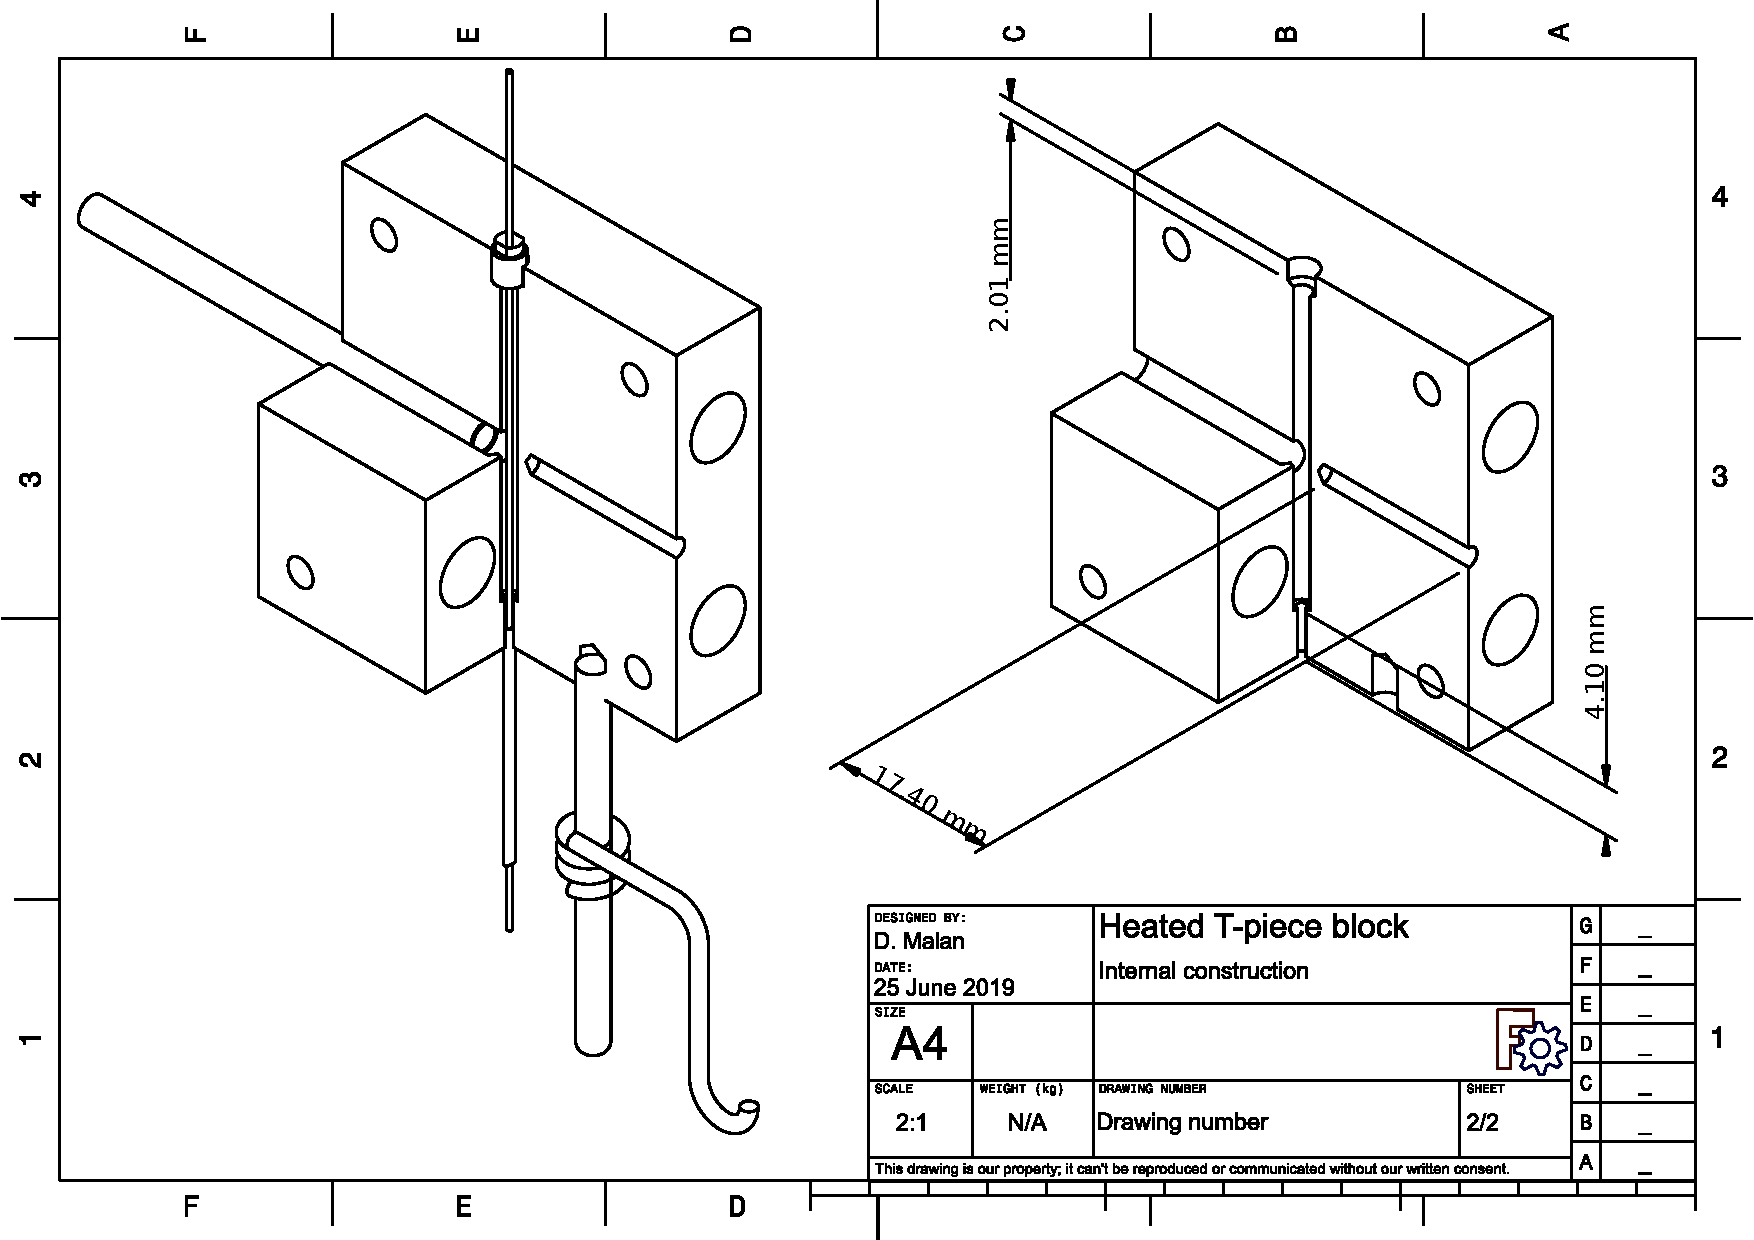
\includegraphics[angle=90, origin=c, width=0.8\textwidth]{./Figures/ManifoldAssemby.pdf}
	\decoRule	
	\caption[Manifold assembly.]{Internal construction and assembly of the heated T-piece blocks}
	\label{fig:ManifoldAssy}
\end{figure}


\subsubsection{Cryogen supply}

Experience taught that for repeatable cooling, the source of liquid carbon
dioxide had to be near the solenoid valve. If this was not the case, when the
valve was opened initially only carbon dioxide gas would be admitted, followed
by a mixture of gas and liquid, and only finally liquid. To solve this problem
we installed a reservoir for liquid carbon dioxide on top of the GC. The problem
of filling a receptacle with liquid carbon dioxide was described in Section
\ref{sec:CO2Pump}. The final design of the reservoir therefore took the form of
a coil of copper tube immersed in a circulating coolant (Figure
\ref{fig:CryogenReservoir}). Mounting the reservoir above the cut-off valve
allows the liquid to collect at the bottom and allow gas to collect at the top,
so that when the valve opens the flow into the coaxial heater contains only
liquid.

\begin{figure}
	\centering
	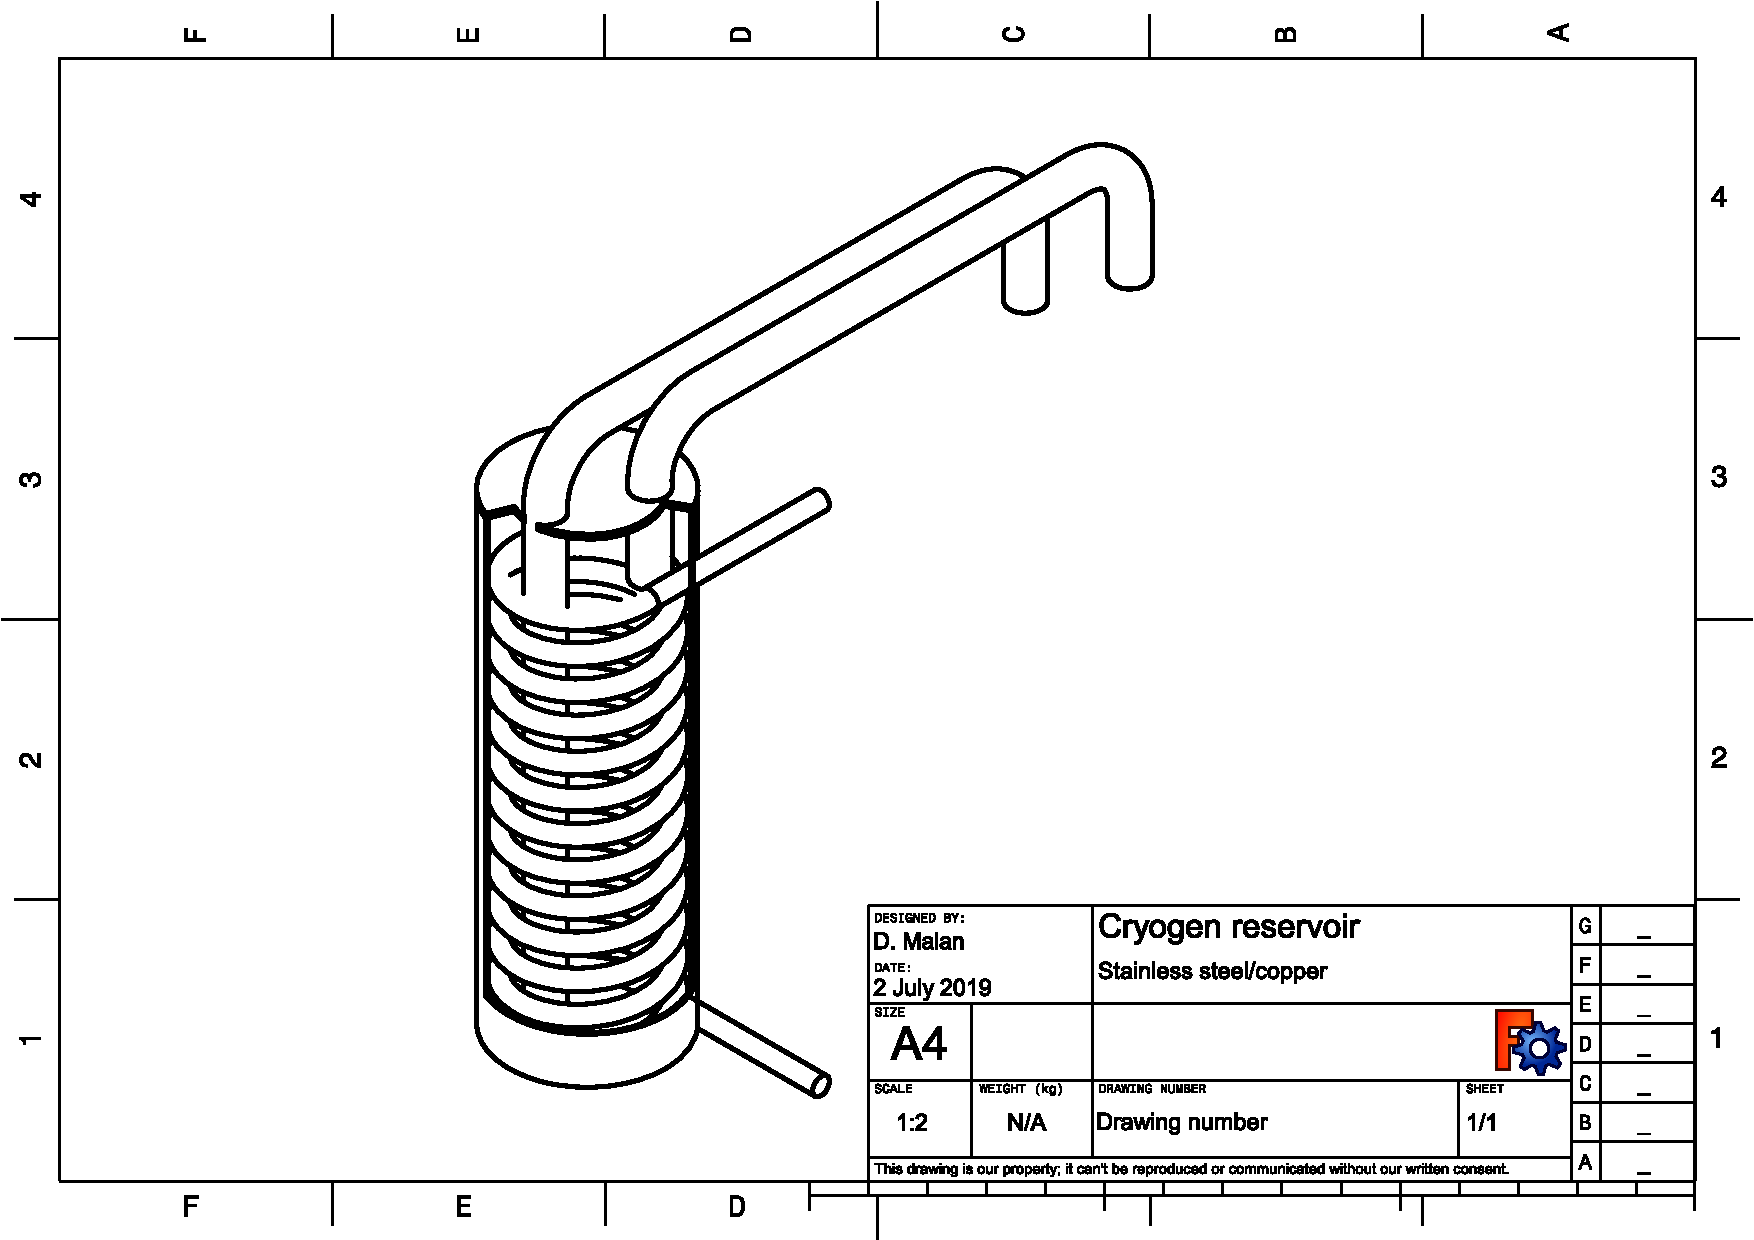
\includegraphics[angle=90, origin=c, width=0.8\textwidth]{./Figures/CryogenReservoir.pdf}
	\decoRule
	\caption[Coolant reservoir]{Cut-away drawing of coolant reservoir.}	
	\label{fig:CryogenReservoir}
\end{figure}


\subsection{Column mounting}

The T-piece blocks described elsewhere\todo{refer to section/page describing
T-piece block} acted as a mounting point for the coaxial heater. The block is
quite heavy, and has to transmit the forces of the coolant tube and the
electrical connections. The column runs from the heated inlet/detector to the
heated T-piece block, and in between it should not be exposed to any
low-temperature cold spots, therefore the gap between the T-piece block and the
inlet/detector should be quite small. But the gap cannot be zero, because
electrical isolation needs to be maintained. A mechanically stiff and accurate
mounting was needed for the T-piece blocks, to allow the precise but
adjustable alignment of the T-piece blocks and the inlet/detector.

Through a few iterations a parallel-rail design was developed. These rails were
held in place in the Varian 3300 oven by friction, so that they could be
adjusted and removed as necessary, yet was stiff enough to transfer the
necessary forces without deflecting. The pointed ends of
the rails pressed against a solid aluminium plate used as the floor of the oven,
and the top, adjustable points pressed against pressure plates which pressed
against the roof of the oven. Figure \ref{fig:RailsDrawing} shows a
technical drawing of the rails as designed. 

\begin{figure}
	\centering
	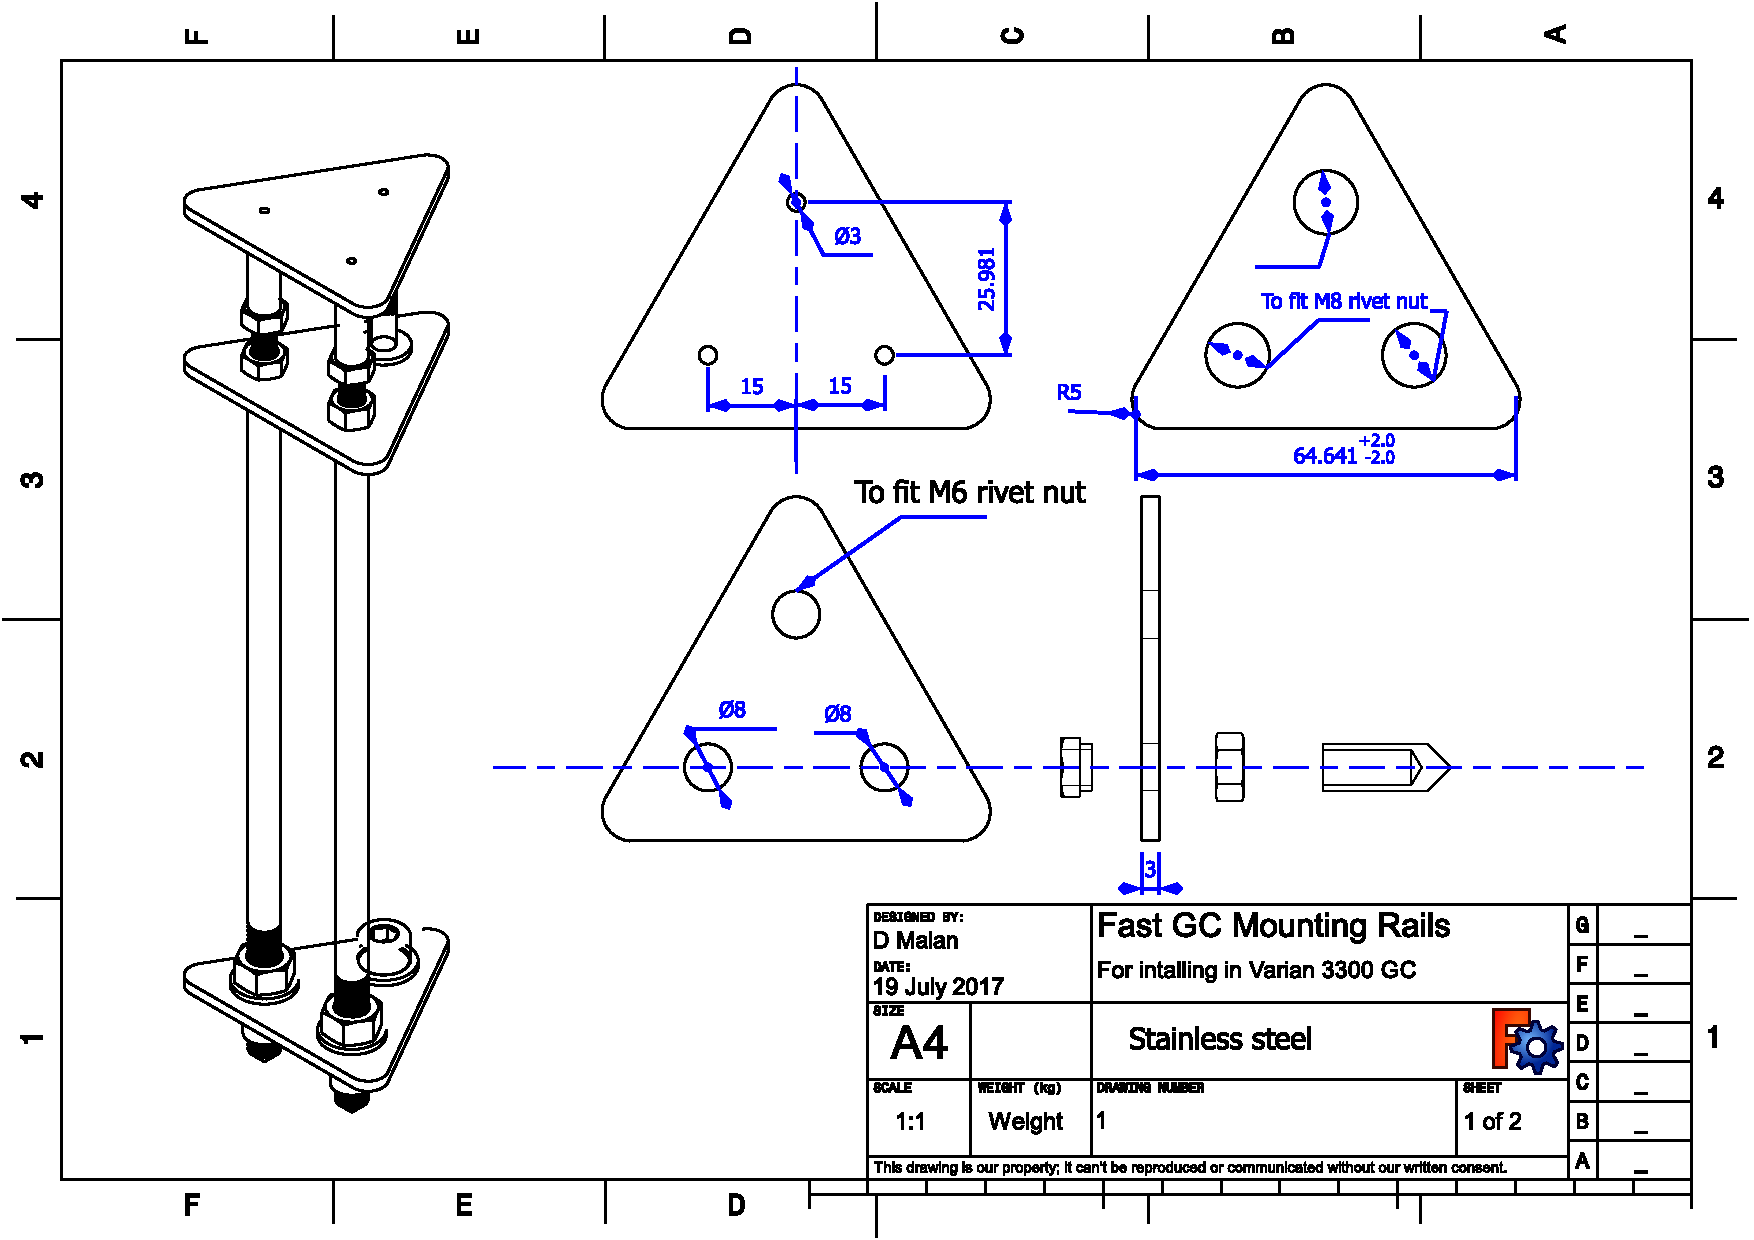
\includegraphics[angle=90, origin=c, scale=0.75]{Figures/RailsDrawing.pdf}
	\decoRule	
\caption[Technical drawing of coaxial heater mounting rails]{\label{fig:RailsDrawing}A technical drawing of the rails carrying the T-piece mounting block.} 
	
\end{figure}

The T-piece blocks was the electrical connection for the resistive coaxial heater,
which meant they needed to be electrically isolated, but they were also heated
which meant that the insulation had to be heat resistant. A commercial available
material that met these requirements was found in the form of \textit{silicon
mica}, a composite material of mica and a silicone resin. This material has a
continuous operating temperature of at least \SI{500}{\celsius}, making it
ideally suited to GC applications. The silicon mica is also easy to machine, so
that it could he shaped to the necessary specifications.

The T-piece blocks were mounted on a pair of cars riding on the round-bar rails.
The cars comprised a sandwich design of layers of stainless steel and silicon
mica around a pair of brass bushes. Once assembled, the cars offered a set of
studs on to which the user could slide and bolt down the T-piece blocks. The
position of the cars were determined by a locking collar on one of the rails.
Figure \ref{fig:CarsDrawing1} shows technical drawings of the cars that explains
the design.

\begin{figure}
	\centering
	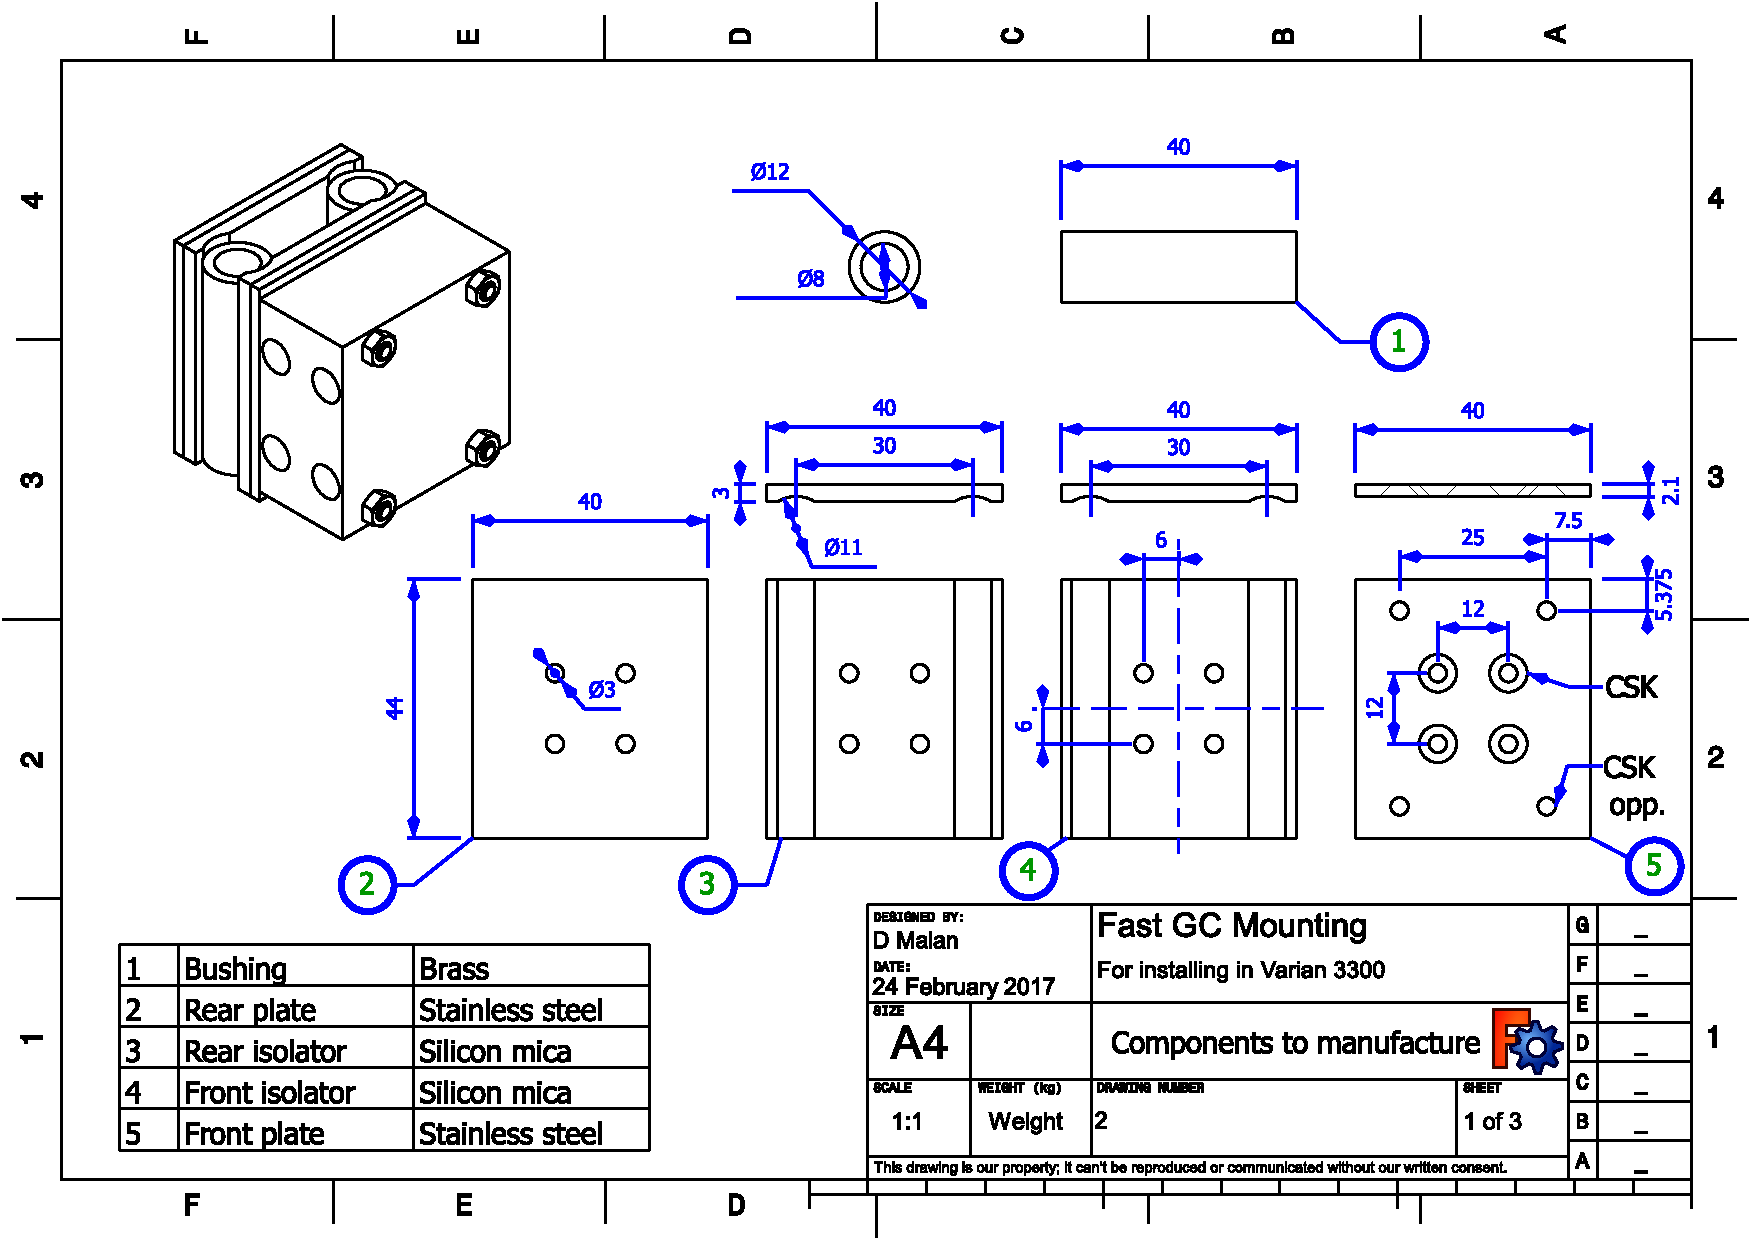
\includegraphics[angle=90, origin=c, width=\textwidth]{Figures/CarDrawing1.pdf}
	\decoRule	
	\caption[Technical drawing of coaxial heater mounting.]{A technical drawing of the T-piece block mounting.} 
	\label{fig:CarsDrawing1}
\end{figure}

\begin{figure}
	\centering
	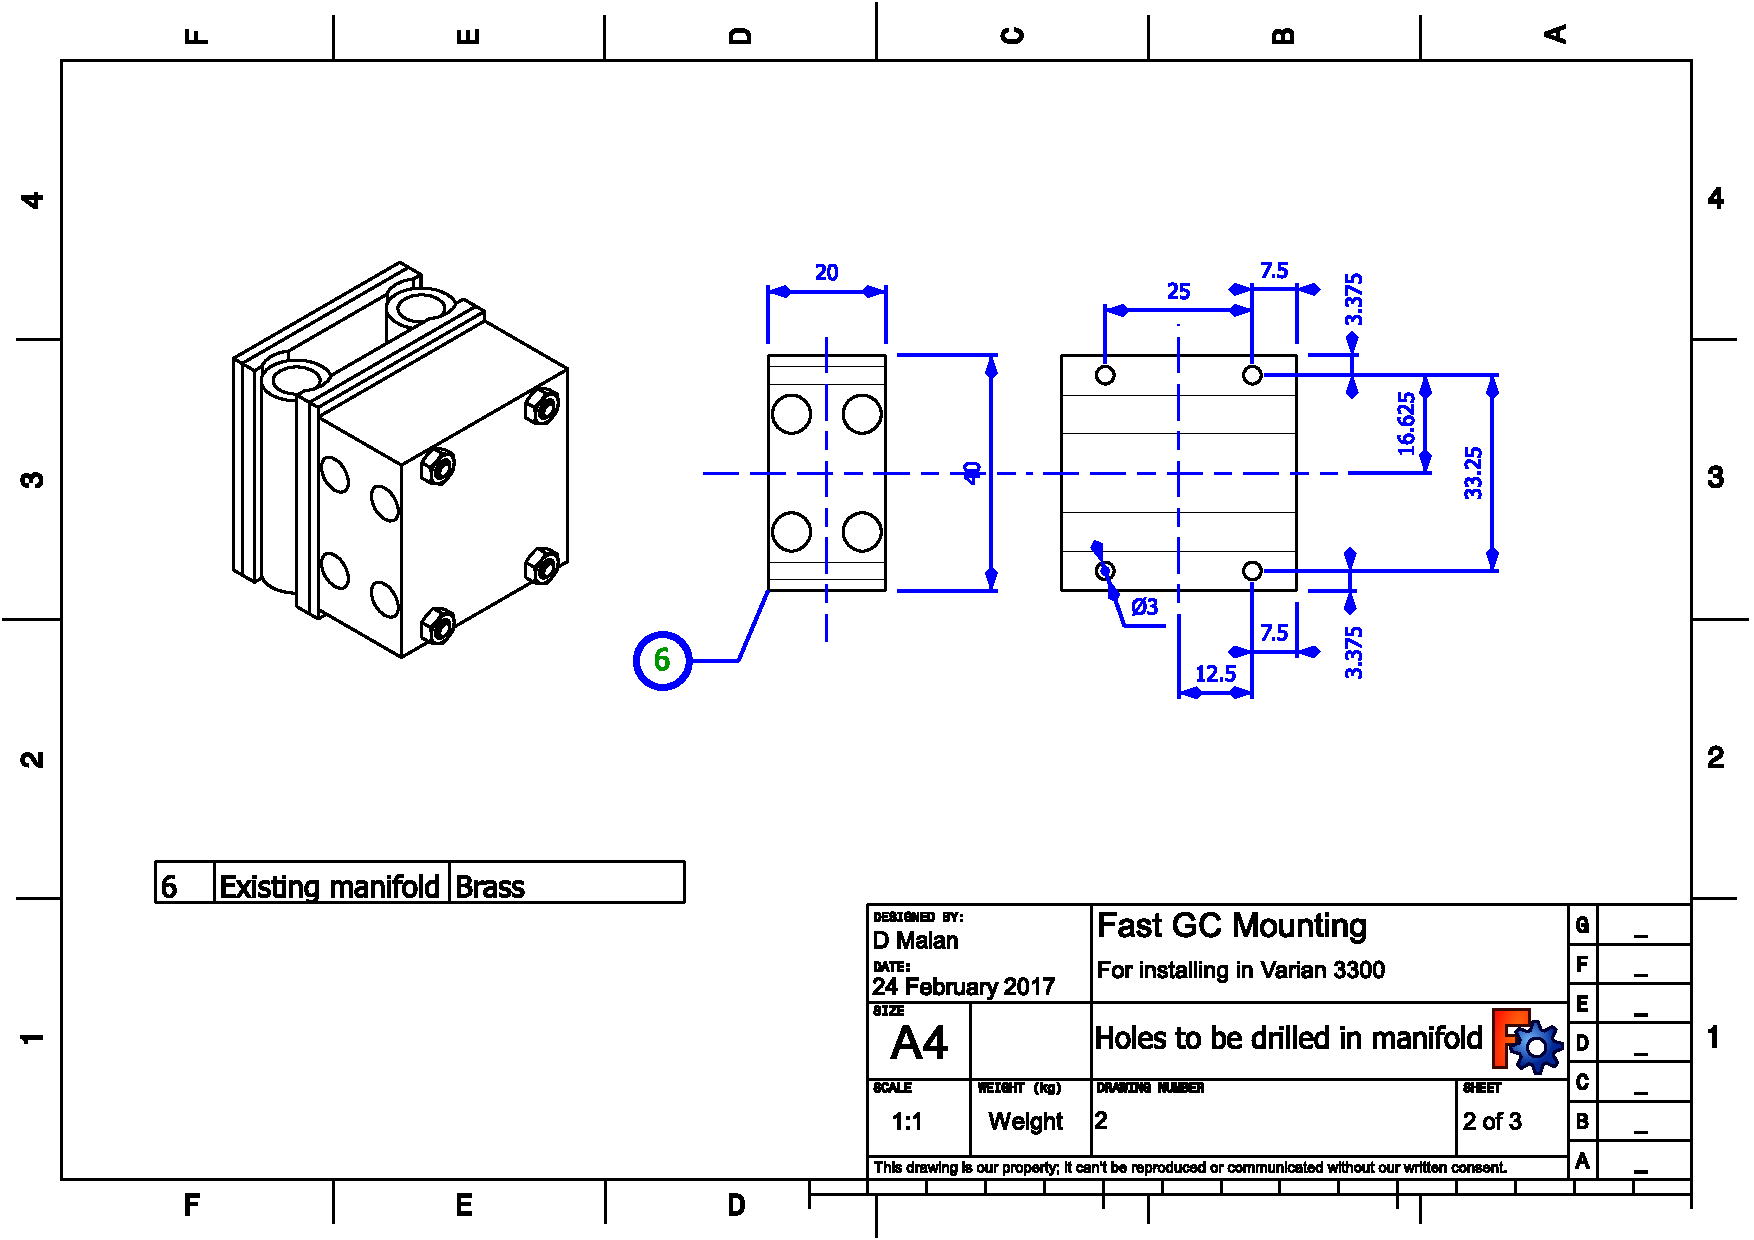
\includegraphics[angle=90, origin=c, width=\textwidth]{Figures/CarDrawing2.pdf}
	\decoRule	
	\caption[Technical drawing of coaxial heater mounting.]{A technical drawing of the T-piece block mounting.} 
	\label{fig:CarsDrawing2}
\end{figure}

\begin{figure}
	\centering
	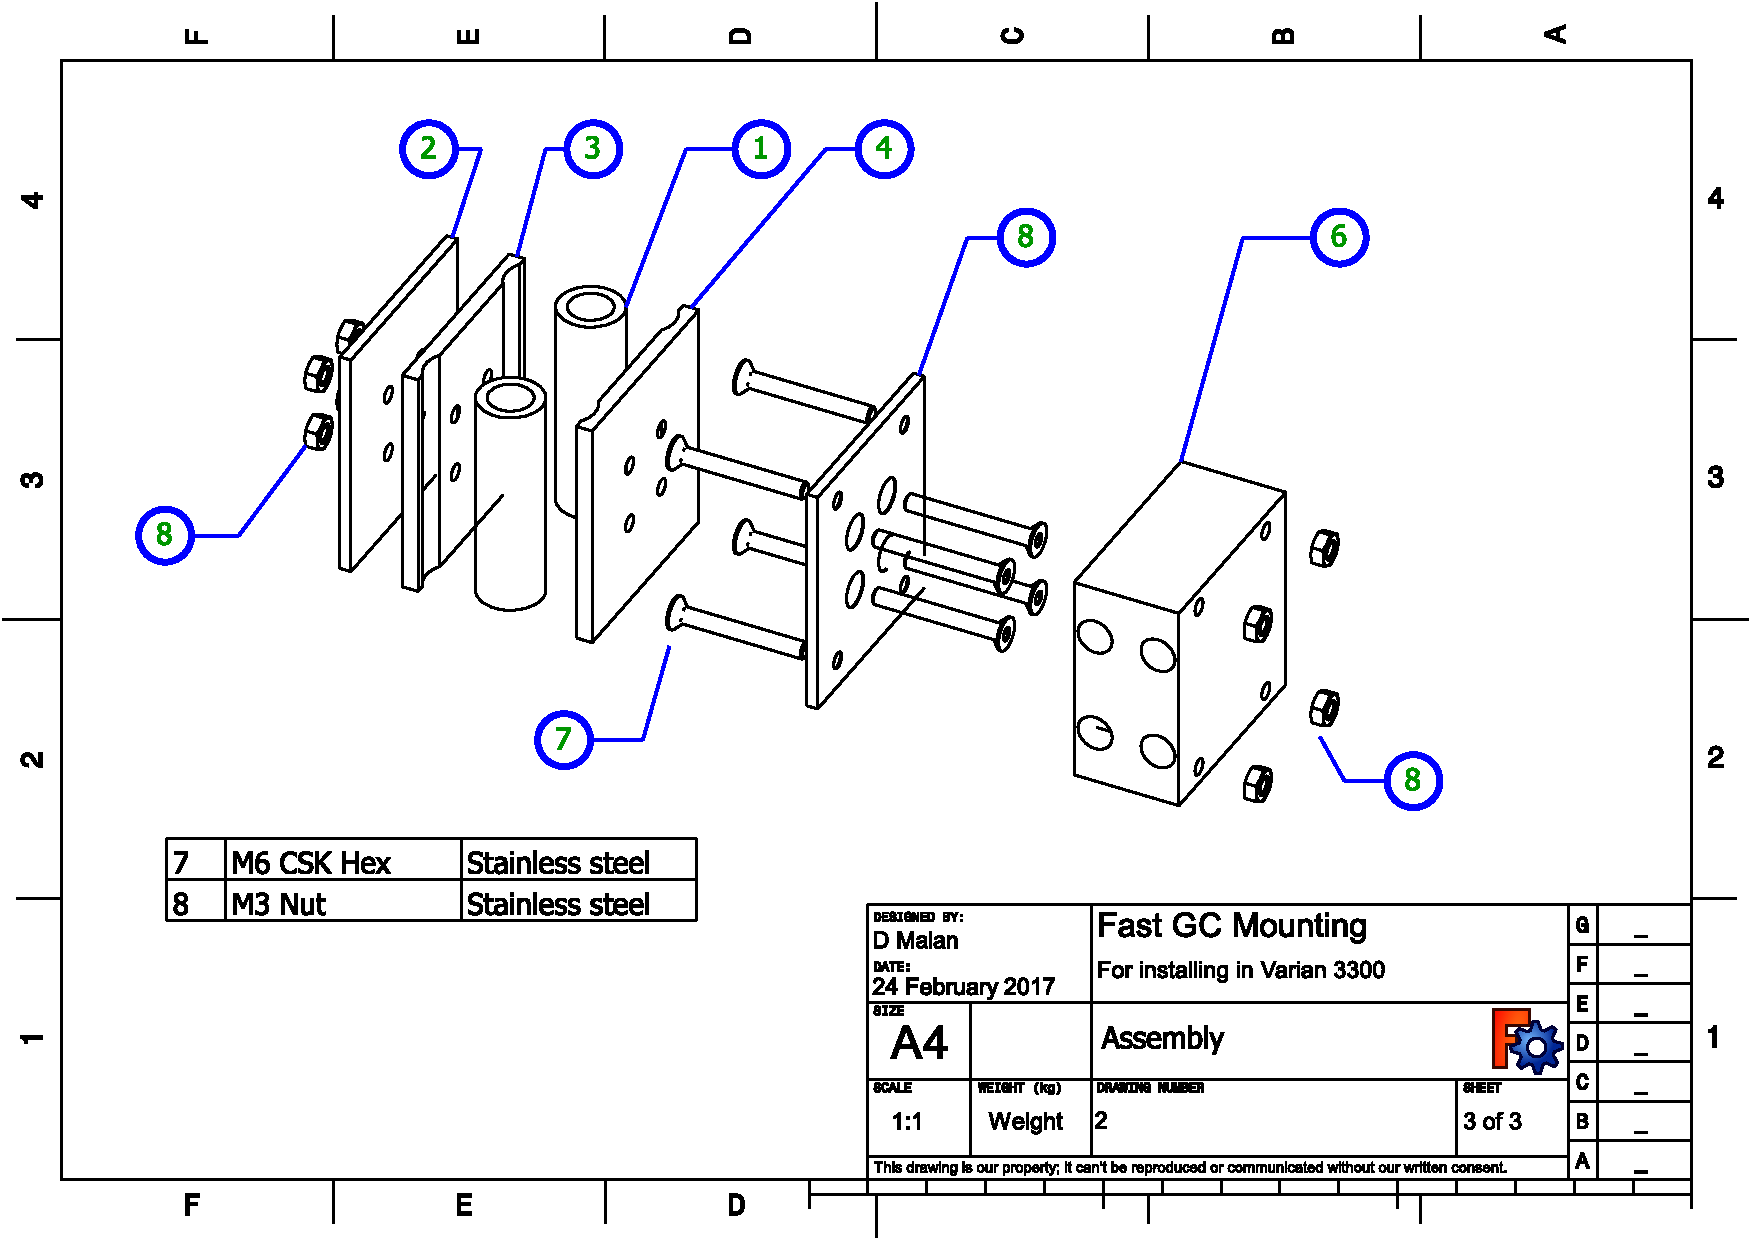
\includegraphics[angle=90, origin=c, width=\textwidth]{Figures/CarDrawing3.pdf}
	\decoRule	
	\caption[Technical drawing of coaxial heater mounting.]{A technical drawing of the T-piece block mounting.} 
	\label{fig:CarsDrawing3}
\end{figure}

\todo{Use Figure environment instead of includepdf. \\
Use caption package to suppress labelling of continued figures \\. 
https://tex.stackexchange.com/questions/64231/how-can-i-create-a-continued-figure-caption}

\subsection{Heating control}

The amount of power supplied to the heater was controlled by a bank of six
transistors in parallel to distribute the heat dissipation.

\subsubsection{Temperature monitoring}

Independent of the amount of power dissipated in the coaxial heater, the current
through the reference resistor was compared to the current through the column.
This ratio corresponds to the resistance of the coaxial heater. This resistance
is a function of the temperature of the heater.

\subsubsection{Loop tuning}

\section{Detector}

The detector used in this fast GC was an unmodified Varian\texttrademark{} 3300
Flame Ionization Detector. The detector bias voltage was supplied by the
original electronics, but a stand-alone high-speed electrometer (V.G. Micromass
Ltd, Model M406-H) captured the signal, which was then conditioned by a
bench-top amplifier (V.G. Micromass Ltd, Model M406) before it was sent to the
computer. This electrometer and amplifier were fast enough to detect and amplify
the signals generated by the fast GC.

\section{Data capture}

In GC×GC, 2D data is recorded as a continuous FID output stream, as if it
is a 1D GC chromatogram, and later converted into a 2D chromatogram, using
knowledge of the modulation period.

For two reasons we could not use this approach. Firstly, in our instrument the
first (SFC) dimension runs in a stop-flow mode making continuous data recording
inappropriate. Secondly, the duration of the cooling cycle varies, which would
introduce unacceptable variation in \textsuperscript{2}D retention times.

We therefore constructed 2D chromatograms by starting to record data each time
the GC fast temperature program started, noting the GC start time as the elution
time of the first (SFC) dimension.

\section{Data visualization}
For data visualization we used the technical computing system Mathematica
11.3\texttrademark{} (Wolfram).  First the collected data was converted to a
list of three-element lists, with $^1$D retention time, $^2$D retention time,
and detector signal as the elements of the inner lists. The Mathematica
functions \texttt{List3DPlot[]} and \texttt{ContourPlot[]} could then be used to
plot 3D chromatograms or contour plots respectively.

\section{Suggested design improvements}

\subsection{Four-wire resistance measurement}
\subsection{Legs heating and cooling integrated in detector and inlet}
\subsection{}

\todos

